\documentclass[reprint,aps,prd,amsmath,amssymb,nofootinbib,floatfix]{revtex4-2}

\usepackage{graphicx}
\usepackage{bm}
\usepackage{mathrsfs}
\usepackage{amsthm}
\usepackage{microtype}
\usepackage[colorlinks=true,linkcolor=blue,citecolor=blue,urlcolor=blue]{hyperref}

\newtheorem{theorem}{Theorem}
\newtheorem{proposition}[theorem]{Proposition}

\newcommand{\scrD}{\mathscr{D}}
\newcommand{\scrA}{\mathscr{A}}
\newcommand{\calH}{\mathcal{H}}
\newcommand{\calA}{\mathcal{A}}
\newcommand{\calB}{\mathcal{B}}
\newcommand{\calK}{\mathcal{K}}
\newcommand{\calM}{\mathcal{M}}
\newcommand{\lP}{\ell_P}
\newcommand{\Tr}{\mathrm{Tr}}
\newcommand{\ethop}{\eth}
\newcommand{\bareth}{\bar{\eth}}

\begin{document}

\title{Fuzzy-Sphere Regularization of Algebraic Null-Cone Quantum Gravity}

\author{Ric Fulop}
\email{ricfulop@mit.edu}
\affiliation{Center for Bits and Atoms, Massachusetts Institute of Technology, Cambridge, MA 02139, USA}
\date{\today}

\begin{abstract}
Chandrasekaran~\cite{Chandrasekaran2026} recently proposed a background-independent Lorentzian quantization of four-dimensional vacuum general relativity on intersecting null cones, obtaining a reduced phase space with corner edge modes, an intrinsic gravitational clock, and an axiomatic bridge between Lorentzian gluing and Euclidean path integrals. We verify directly that the classical first-order null-cone reduction holds identically and that the conditional Lorentzian-to-Euclidean equivalence theorem is sound once its axioms are met. When quantized directly in the continuum, however, the proposal meets four obstructions: non-trace-class counterexamples and circularity in the finiteness arguments, vacuum collapse of the unrenormalized focusing clock together with divergence of the inverse lapse, a quadratic angular divergence in the four-dimensional graviton pair-creation amplitude, and a two-loop divergence for any regulator acting only on the transverse sphere. We show that these obstructions can be resolved without altering the classical null-cone structure by introducing three microscopic ingredients: compact $SU(2)$-equivariant fuzzy monopole bundles with a parity-symmetrized matrix action $I_{\mathrm{FSG}}^{(N)}$, a smoothly smeared normal-ordered gravitational clock bounded by massive quantum energy inequalities and Fredholm determinants, and an area-scaled double-null occupation budget $\sum n_{k,j,m,p}(k+t_j^2/k)\le B(s)=s Q_*$. Under the projected Hamiltonian $H_{\mathrm{phys}}=P_{B(s)}H_{\mathrm{FSG}}P_{B(s)}$, every fixed-area Hilbert space and fixed-budget perturbative sum is finite without circularity while preserving the macroscopic $s^{-3/2}$ and $s^{-2}\ln s$ pair-creation asymptotics. Coupling discrete corner states to the fuzzy-sphere radiative sector reproduces universal four-dimensional one-loop logarithmic corrections across Schwarzschild, flat space, and de Sitter space, yields the $\mathrm{AdS}_4$ Hawking--Page transition and Don Page's graviton Hawking luminosity, and provides finite-dimensional realizations of baby-universe factorization and semiclassical backreaction. Finally, a nonperturbative hybrid Monte Carlo study of the matrix path integral up to rank $N=48$ ($1.33\times 10^6$ degrees of freedom) shows that the invariant DeWitt--Fujikawa spin-2 measure stabilizes a smooth, caustic-free geometric phase with massless gravitons and strong $N$-independent suppression of non-spherical horizon roughness, whereas the flat measure triggers radiative horizon collapse.
\end{abstract}

\maketitle

\section{Introduction}\label{sec:intro}

In perturbative quantum gravity one expands the metric around a fixed background spacetime and quantizes small fluctuations. Nonperturbatively, background independence requires observables defined without reference to any chosen background, for example by dressing bulk fields to gravitational data on the boundary of a finite subregion. Recent work on characteristic initial-value formulations~\cite{ChoquetBruhat2011,Reisenberger2008,Reisenberger2013}, gravitational edge modes and corner symmetries~\cite{DonnellyFreidel2016,FreidelGeillerPranzetti2020,ChandrasekaranFlanagan2023,CiambelliFreidelLeigh2024,CiambelliKlinger2026}, subregion von Neumann algebras~\cite{CLPW2023,CPW2023}, and axiomatic gravitational path integrals~\cite{CDMW2024} points to the null cone as a natural setting for this problem, because the gravitational constraints reduce to ordinary differential equations along null generators.

In Ref.~\cite{Chandrasekaran2026}, Venkatesa Chandrasekaran combined these ingredients into a proposal for four-dimensional vacuum general relativity on intersecting null cones. Starting from first-order Pleba\'nski gravity, Ref.~\cite{Chandrasekaran2026} solves the constraints at finite $G_N$ with corner edge modes, isolates a canonical symplectic form and a boundary-localized reduced Hamiltonian $H_c$, and introduces an intrinsic gravitational clock built from null Raychaudhuri focusing. Using this clock to dress a causal diamond $\scrD$, Ref.~\cite{Chandrasekaran2026} links corner area directly to boost-generated traces, Bekenstein--Hawking entropy, Sen's one-loop logarithmic correction~\cite{Sen2013}, and spatial-topology null states~\cite{MarolfMaxfield2020}. Appendix~E of Ref.~\cite{Chandrasekaran2026} further formulates five Lorentzian cobordism axioms and establishes a conditional equivalence with the Euclidean reflection-positive framework of Ref.~\cite{CDMW2024}, identifying replica traces with traces in a Type~I algebra without assuming $\mathrm{AdS}/\mathrm{CFT}$.

Because this framework aims to derive finite-dimensional subregion Hilbert spaces, ultraviolet-finite transition amplitudes, one-loop black hole entropy corrections, and the semiclassical Einstein equations directly in the continuum, its mathematical foundations warrant careful examination. We have checked both the classical derivation and the quantum arguments of Ref.~\cite{Chandrasekaran2026} through direct symbolic calculation, numerical analysis, and formal proof checking. Our findings separate cleanly into two parts. The classical first-order null-cone reduction (Sec.~3 and Appendices~A and~B of Ref.~\cite{Chandrasekaran2026}) holds identically across all fourteen core identities, and the conditional Lorentzian-to-Euclidean equivalence theorem (Appendix~E.2) is valid once Axioms~1--5 are satisfied. By contrast, promoting this structure directly to the continuum (Secs.~4 and~5 and Appendix~E.3) runs into four independent obstructions that prevent the continuum ansatz from satisfying Axioms~1--5.

Our aim here is constructive. We preserve Chandrasekaran's classical null-cone phase space and axiomatic architecture while resolving all four obstructions through three microscopic ingredients:
\begin{enumerate}
\item \emph{Fuzzy monopole bundles on the corner:} we replace continuum two-spheres with compact $SU(2)$-equivariant rectangular matrix bundles $\calB_{s_w}^{(N)}$ of dimension $N^2-s_w^2$ ($s_w\in\{0,\pm 1,\pm 2\}$), equipped with an explicit $SU(2)$-equivariant embedding map $\iota_{N\to M}$ and a parity-symmetrized $SU(N)$ null-cone action $I_{\mathrm{FSG}}^{(N)}$ free of spurious low-angular-momentum or higher-spin fields.
\item \emph{A smoothly smeared normal-ordered gravitational clock:} we replace the sharp-endpoint, unrenormalized focusing operator $\widehat{\Xi}_y(1)$ by a normal-ordered Raychaudhuri integral smeared with a compactly supported smooth function $g\in C^\infty_c((0,1))$, which we bound uniformly across all four-dimensional spin-2 harmonics using the Fewster--Eveson massive quantum energy inequality~\cite{Flanagan1997,FewsterEveson1998} and Balian--Br\'ezin Fredholm determinants~\cite{BalianBrezin1969}.
\item \emph{An area-scaled double-null occupation budget:} we impose the total occupation constraint $\sum_{k,j,m,p} n_{k,j,m,p}(k+t_j^2/k)\le B(s)=s Q_*$, with $t_j^2=\frac{1}{2}(j-1)(j+2)$, which bounds radial frequencies, angular momenta, and bosonic occupation numbers simultaneously while preserving macroscopic non-analytic behavior.
\end{enumerate}

We organize the remainder of the paper as follows. In Sec.~\ref{sec:audit} we summarize our verification of the classical null-cone reduction and state the four continuum obstructions. In Sec.~\ref{sec:unified} we construct the fuzzy-sphere null-cone action $I_{\mathrm{FSG}}^{(N)}$ (written in full in Appendix~\ref{app:explicit_action}), its parity-symmetrized cubic vertices in closed Wigner-$6j$ form, the massive-QEI clock and exponential-clock bounds, the projected physical Hamiltonian $H_{\mathrm{phys}}=P_{B(s)}H_{\mathrm{FSG}}P_{B(s)}$, the second-variation emergence of Regge--Wheeler and Zerilli dynamics, sub-Planckian $SO(3,1)$ boost closure, and Ermakov--Pinney caustic regularization. In Sec.~\ref{sec:1loop} we derive the Lichnerowicz curvature decomposition and a four-dimensional infrared isotropy theorem, reproducing the universal one-loop logarithmic corrections on Schwarzschild, flat space, and de Sitter $S^4$. In Sec.~\ref{sec:uv} we analyze the two-loop regulator behavior, compute the Schwarzschild Goroff--Sagnotti entropy shift alongside a sub-Planckian pixel-size naturalness ceiling ($s_{\min}\le\pi$), sum dynamically over matrix ranks $N$ to recover the $\mathrm{AdS}_4$ Hawking--Page transition, and test $SU(2)$-singlet corner fusion on a three-diamond network. In Sec.~\ref{sec:orig_sections} we present finite-dimensional realizations of Secs.~4.4, 5.4, and~6 of Ref.~\cite{Chandrasekaran2026}. In Sec.~\ref{sec:hmc} we report a nonperturbative hybrid Monte Carlo study of the Euclidean matrix path integral up to rank $N=48$. We close in Sec.~\ref{sec:discussion} with open dynamical questions; Appendix~\ref{app:code} catalogs our machine-checked formal proofs and publicly archived numerical code.

\section{Audit of the Continuum Quantization}\label{sec:audit}

\subsection{Classical Null-Cone Reduction and Axiomatic Bridge}\label{sec:audit_pass}

Before introducing any regularization, we reconstructed the four-dimensional null-cone metric, spin connection, Ricci curvature, constraint kernels, boundary terms, and Iyer--Wald charges of Sec.~3 and Appendices~A and~B of Ref.~\cite{Chandrasekaran2026} by direct symbolic computation. All fourteen core classical identities hold identically: the null-cone symplectic form (Eqs.~3.39--3.42d), tetrad spin-connection components (Eq.~A.1), linearized Raychaudhuri Green's function jump (Eqs.~A.23d--A.27), $V$-coordinate constraint kernel and second-class inverse (Eqs.~A.30b--A.36), triangular symplectic decoupling (Eqs.~A.37--A.41), the Raychaudhuri, Damour--Navier--Stokes, and cross-focusing equations (Eqs.~B.3--B.5c), the bulk Hamiltonian divergence identity (Eq.~B.7), displaced null-boundary inaffinity (Eqs.~B.8d--f), the Einstein--Hilbert boundary decomposition (Eqs.~B.10--B.12), and the Iyer--Wald Noether charge on a displaced cut (Eq.~B.17).

We also checked the logical dependency structure of Appendix~E.2 formally (Appendix~\ref{app:code}). Conditionally on Lorentzian Axioms~1--5 (diffeomorphism invariance, reflection positivity, factorization, continuous unitary evolution, and spectral trace finiteness), the analytic continuation of boundary time translations to Euclidean cylinders and the isometric equivalence with the Euclidean Type~I boundary algebra of Ref.~\cite{CDMW2024} follow without logical gaps. Chandrasekaran's classical phase space and conditional axiomatic equivalence therefore stand intact.

\subsection{Four Continuum Obstructions}\label{sec:audit_fail}

Promoting this structure directly to the continuum in Secs.~4 and~5 encounters four independent mathematical obstructions.

\begin{theorem}[Continuum Obstructions]\label{thm:nogo}
In the strict continuum null-cone quantization of Ref.~\cite{Chandrasekaran2026}, the following four obstructions occur:
\begin{enumerate}
\item \emph{Non-entailment and circularity in Sec.~5.2:} Open-amplitude Cauchy--Schwarz bounds (Eq.~4.30) do not imply trace-class convergence of closed traces. Without assuming closed-trace convergence, the hypotheses of Sec.~5.2 admit infinite-dimensional countermodels (both $\calH=\mathbb{C}^2\otimes\ell^2(\mathbb{N})$ and a discretized bounded-dilaton JT model coupled to a massless scalar) with $\dim\calH_{\scrD}=\infty$ and $Z_\beta=\infty$. Conversely, assuming closed-trace convergence renders the boost-and-cycle argument redundant and creates a logical circle between Sec.~5.2 and Appendix~E.3.
\item \emph{Vacuum collapse of the focusing clock and lapse singularity:} Symplectic diagonalization of the unrenormalized focusing operator $\widehat{\Xi}_y(v)$ (Eq.~4.22) produces a ground-state zero-point energy growing as $E_{0,\min}\sim 14.64\,N_{\mathrm{rad}}^2 J^2/s$. Beyond mode count $N_\star\sim [s\ln(\ell/u_{\mathrm{cl}})/14.64]^{1/4}$, this collapses the clock projector identically to $P_{\scrD}\equiv 0$ and drives the inverse lapse $N(\epsilon,y)^{-1}=N(1,y)^{-1}\exp(\widehat{\Xi}_y(1))\to+\infty$ inside $H_c$ (Eqs.~3.54--3.55). Naive Wick normal ordering restores finiteness only by allowing negative expectation values in squeezed states ($\langle r|{:}(\hat{a}+\hat{a}^\dagger)^2{:}|r\rangle=e^{-2r}-1<0$), violating the area upper bound Eq.~(5.21d).
\item \emph{Angular divergence in Sec.~4.4 and non-unique gluing:} Restoring all $2[(J+1)^2-4]$ angular graviton modes to the one-dimensional pair-creation sum $\mathrm{Li}_2(e^{-2i/s})/(2s^2)$ of Sec.~4.4 causes the amplitude to diverge quadratically ($\propto J^2$) even at fixed $G_N$. Independently, Kadison--Singer pure-state extensions leave area-changing gluing matrix elements $\omega(U_{\calM})\in[-1,1]$ undetermined by the fixed-area subalgebra.
\item \emph{Microscopic state deficit and two-loop transverse-only divergence:} Using the Weyl mode count $\#\{\nu_i\le\nu\}=(s\nu)^3$ of Appendix~D.3 (Eq.~D.45a), perturbative continuum gravitons inside a focusing budget $Q_*$ yield only $\ln d(s)\approx c_{\mathrm{SB}}(sQ_*)^{3/4}\ll s$ with $c_{\mathrm{SB}}=\frac{4}{3}(\pi^4/5)^{1/4}=2.801$, an exponentially small fraction of $e^s$. Moreover, the squashed-cone Gauss--Bonnet proxy disagrees with the covariant one-loop gravity heat kernel~\cite{BBM2022,FPS2013} by $-112\pi^2/5$ on a round Minkowski sphere (though the $k^2$ term vanishes on a marginally trapped surface), and regulating only the transverse $S^2$ fails at two loops ($\sim \Lambda_\parallel^2\ln\Lambda_\parallel$, Sec.~\ref{sec:uv_2loop}).
\end{enumerate}
\end{theorem}

The quantitative witnesses behind Theorem~\ref{thm:nogo} are explicit. On $\calH=\mathbb{C}^2\otimes\ell^2(\mathbb{N})$ with $s\in\{0,2\pi\}$, $C_b=\mathrm{diag}(1,e^{-\pi})\otimes\hat{1}$, and boost $\eta=\pi$ ($\delta_\eta=0.172533$), a product exhaustion gives $Z_{P_M}[X]=+0.086428\,M\to+\infty$ whereas a length-$200$ cycle exhaustion gives $Z_{P_{\mathrm{cyc}}}[X]\le -16.9944\,K\to-\infty$, while still satisfying Eq.~(5.32) with $\langle\Delta_\pi\widehat{\mathcal{O}}\rangle_P\le 0.00087\ll\delta_\eta/2$. For the $\mathrm{AdS}$ thermal sum in Eqs.~(5.44)--(5.45), unconditional convergence of finite-subset differences holds if and only if $\sum_i w_i<\infty$. On a macroscopic causal diamond ($s=\pi\times 10^{10}$, $\ell(\scrD)=10\,u_{\mathrm{cl}}$), Williamson diagonalization gives $E_{0,\min}=29.25$ ($u_{\min}/u_{\mathrm{cl}}=5.04\times 10^{12}$, $P_{\scrD}\equiv 0$) at mode cutoff $N_{\mathrm{rad}}=J=500$, and $E_{0,\min}=467.0$ ($N^{-1}\ge 6.81\times 10^{202}$) at $N_{\mathrm{rad}}=J=1000$. In physical units, the unrenormalized clock breaks down far below the Planck energy, already near $43.7\,\mathrm{GeV}$ for a $1\,\mathrm{m}$ tabletop diamond and $0.80\,\mathrm{GeV}$ for a solar-mass black hole.

\section{Fuzzy-Sphere Null-Cone Matrix Gravity}\label{sec:unified}

To overcome all four obstructions while retaining the classical phase space of Ref.~\cite{Chandrasekaran2026}, we lift the null-cone fields onto a fuzzy sphere of dynamically determined matrix rank, replace the sharp clock by a smoothly smeared massive-QEI clock, and impose an area-scaled double-null occupation budget.

\subsection{Fuzzy Monopole Bundles, Explicit Matrix Vertices, and the Action $I_{\mathrm{FSG}}^{(N)}$}\label{sec:unified_action}

At corner dimensionless area $s=\scrA/(4G_N\hbar)=M s_{\min}$ built from elementary area quanta (embadons), we set the fuzzy-sphere rank to $N=J_{\max}(s)+1\le\lfloor\sqrt{s/s_{\min}}\rfloor+1$. Rather than embedding gravity inside a Yang--Mills matrix model, which introduces unwanted higher-spin towers~\cite{Steinacker2026}, we represent each Bondi--Sachs field of spin weight $s_w\in\{0,\pm 1,\pm 2\}$ directly as a rectangular matrix in the $SU(2)$-equivariant fuzzy monopole bundle
\begin{equation}\label{eq:fuzzy_bundle}
\calB_{s_w}^{(N)} \;=\; \mathrm{Hom}\!\left(V_{\frac{N-1-s_w}{2}},\, V_{\frac{N-1+s_w}{2}}\right) \;\cong\; \bigoplus_{j=|s_w|}^{N-1} V_j,
\end{equation}
of dimension $\dim\calB_{s_w}^{(N)}=(N+s_w)(N-s_w)=N^2-s_w^2$. Scalars ($\widehat{\rho}^2,\widehat{N},\widehat{F}\in\calB_0^{(N)}$) are $N\times N$ Hermitian matrices ($j=0\dots N-1$); complex shift and H\'aji\v{c}ek one-forms ($\widehat{V},\widehat{w}\in\calB_{+1}^{(N)}$) are $(N+1)\times(N-1)$ matrices ($j=1\dots N-1$); and spin-2 shear data ($\widehat{Z}\in\calB_{+2}^{(N)}$) are $(N+2)\times(N-2)$ matrices ($j=2\dots N-1$). By construction, $\calB_{s_w}^{(N)}$ carries no spurious $j<|s_w|$ modes and no $|s_w|>2$ fields.

The $SU(2)$-intertwining fuzzy Newman--Penrose ladder operators $\widehat{\ethop}:\calB_{s_w}^{(N)}\to\calB_{s_w+1}^{(N)}$ and $\widehat{\bareth}:\calB_{s_w}^{(N)}\to\calB_{s_w-1}^{(N)}$ satisfy
\begin{align}\label{eq:fuzzy_eth}
[\widehat{\bareth},\widehat{\ethop}] &= 2 s_w\,\mathrm{Id}, \nonumber\\
-\widehat{\ethop}\widehat{\bareth}\big|_{\calB_2^{(N)}} &= L^2 - 2 = (j-1)(j+2) = 2 t_j^2,
\end{align}
preserving the round-sphere curvature $R[S^2]=+2$ at every finite $N\ge 3$.

To lift nonlinear interactions from Appendix~B of Ref.~\cite{Chandrasekaran2026} into matrix notation, we must specify how an $N\times N$ scalar $F\in\calB_0^{(N)}$ contracts with rectangular products such as $Z^\dagger Z\in\mathrm{End}(\mathbb{C}^{N-2})$ and $Z Z^\dagger\in\mathrm{End}(\mathbb{C}^{N+2})$ for $Z\in\calB_{+2}^{(N)}$. Let $\{T^{(0,M)}_{j,m}\}_{j=0}^{M-1}$ be the canonical orthonormal fuzzy spherical harmonic basis of $\mathrm{End}(\mathbb{C}^M)$, normalized by $\frac{1}{M}\Tr_M(T^{(0,M)\dagger}_{j,m}T^{(0,M)}_{j',m'})=\delta_{jj'}\delta_{mm'}$. We define the unique $SU(2)$-equivariant isometric embedding/projection map $\iota_{N\to M}:\mathrm{End}(\mathbb{C}^N)\to\mathrm{End}(\mathbb{C}^M)$ by
\begin{align}\label{eq:iota_map}
\iota_{N\to M}(F) := \sum_{j=0}^{\min(N,M)-1}\sum_{m=-j}^{j}\!&\left(\frac{1}{N}\Tr_N\!\big[T^{(0,N)\dagger}_{j,m}\,F\big]\right) \nonumber\\
&\times T^{(0,M)}_{j,m}.
\end{align}
With Eq.~\eqref{eq:iota_map}, the parity-symmetrized cubic interaction corresponding to $\int_{S^2} F\,Z_2^* Z_3\,\frac{d\Omega}{4\pi}$ is completely specified in matrix form as
\begin{align}\label{eq:cubic_vertex}
\mathcal{V}_3^{(N)}[F;Z_2,Z_3]
&:= \frac{1}{2\sqrt{N^2-4}}\Big[\Tr_{N-2}\!\big(\iota_{N\to N-2}(F)\,Z_2^\dagger Z_3\big) \nonumber\\
&\quad + \Tr_{N+2}\!\big(\iota_{N\to N+2}(F)\,Z_3 Z_2^\dagger\big)\Big] \nonumber\\
&= \frac{1}{N}\Tr_N\!\big(F\,\mathcal{S}_N^{(2)}(Z_2^\dagger,Z_3)\big),
\end{align}
where $\mathcal{S}_N^{(2)}(Z_2^\dagger,Z_3)=\frac{1}{2\sqrt{N^2-4}}[(N-2)\iota_{N-2\to N}(Z_2^\dagger Z_3)+(N+2)\iota_{N+2\to N}(Z_3 Z_2^\dagger)]\in\calB_0^{(N)}$. Evaluating Eq.~\eqref{eq:cubic_vertex} on basis harmonics $T^{(0,N)}_{j_1 m_1}$ and $T^{(+2,N)}_{j_2 m_2},T^{(+2,N)}_{j_3 m_3}$ gives the closed-form Wigner-$6j$ cubic vertex (with $j_L=\frac{N+1}{2}$ and $j_R=\frac{N-3}{2}$):
\begin{align}\label{eq:wigner6j}
&|C^{(N)}_{j_1 m_1;j_2 m_2;j_3 m_3}|
= \frac{1}{2}\sqrt{(2j_1+1)(2j_2+1)(2j_3+1)} \nonumber\\
&\quad\times \left|\begin{pmatrix}j_1&j_2&j_3\\m_1&-m_2&m_3\end{pmatrix}\right|
\Bigg|\sqrt{N-2}\begin{Bmatrix}j_1&j_2&j_3\\j_L&j_R&j_R\end{Bmatrix} \nonumber\\
&\qquad + (-1)^{j_1+j_2+j_3}\sqrt{N+2}\begin{Bmatrix}j_1&j_2&j_3\\j_R&j_L&j_L\end{Bmatrix}\Bigg|.
\end{align}
Direct matrix evaluation confirms both the adjoint relation~\eqref{eq:cubic_vertex} and Eq.~\eqref{eq:wigner6j} to machine precision ($\sim 10^{-14}$), along with exact $SU(2)$ invariance. Parity symmetrization cancels the $O(1/N)$ shift present in one-sided traces $\Tr_{N-2}(\iota(F)Z^\dagger Z)$ ($p=1.06$), yielding $O(1/N^2)$ convergence to the continuum spin-weighted Gaunt integral ($p=2.05$ for $(2,2,2)$), as shown in Fig.~\ref{fig:v2}(a).

The full operator-ordered matrix action $I_{\mathrm{FSG}}^{(N)}[\widehat{\rho}^2,\widehat{N},\widehat{F},\widehat{V},\widehat{Z}]$ built from $\mathcal{S}_N^{(1)}$ and $\mathcal{S}_N^{(2)}$ is given explicitly in Appendix~\ref{app:explicit_action}. Varying $I_{\mathrm{FSG}}^{(N)}$ reproduces four-dimensional Schwarzschild and Schwarzschild--de Sitter as exact finite-$N$ saddles at every $N\ge 3$ (residual $\le 3.8\times 10^{-16}$). For non-spherical solutions, slow-rotation Kerr $O(a^2)$ quadrupole backreaction and nonlinear $j=2$ gravitational-wave shear focusing conserve the monopole identically ($c_0=1.000000$) and converge to continuum general relativity at order $O(1/N^2)=O(\lP^2/\scrA)=O(1/s)$ ($p=2.00$ for Kerr, $p=2.03$ for shear waves), as shown in Fig.~\ref{fig:unified}(a). In the present formulation, the discrete corner Hilbert space $\calH_{\mathrm{corner}}(M)$ of area $s_M=M s_{\min}$ is coupled kinematically to the radiative matrix action $I_{\mathrm{FSG}}^{(N)}$; deriving the discrete corner spectrum directly from a nonperturbative quantization of $I_{\mathrm{FSG}}^{(N)}$ remains an open problem (Sec.~\ref{sec:discussion}).

\begin{figure*}[t]
\centering
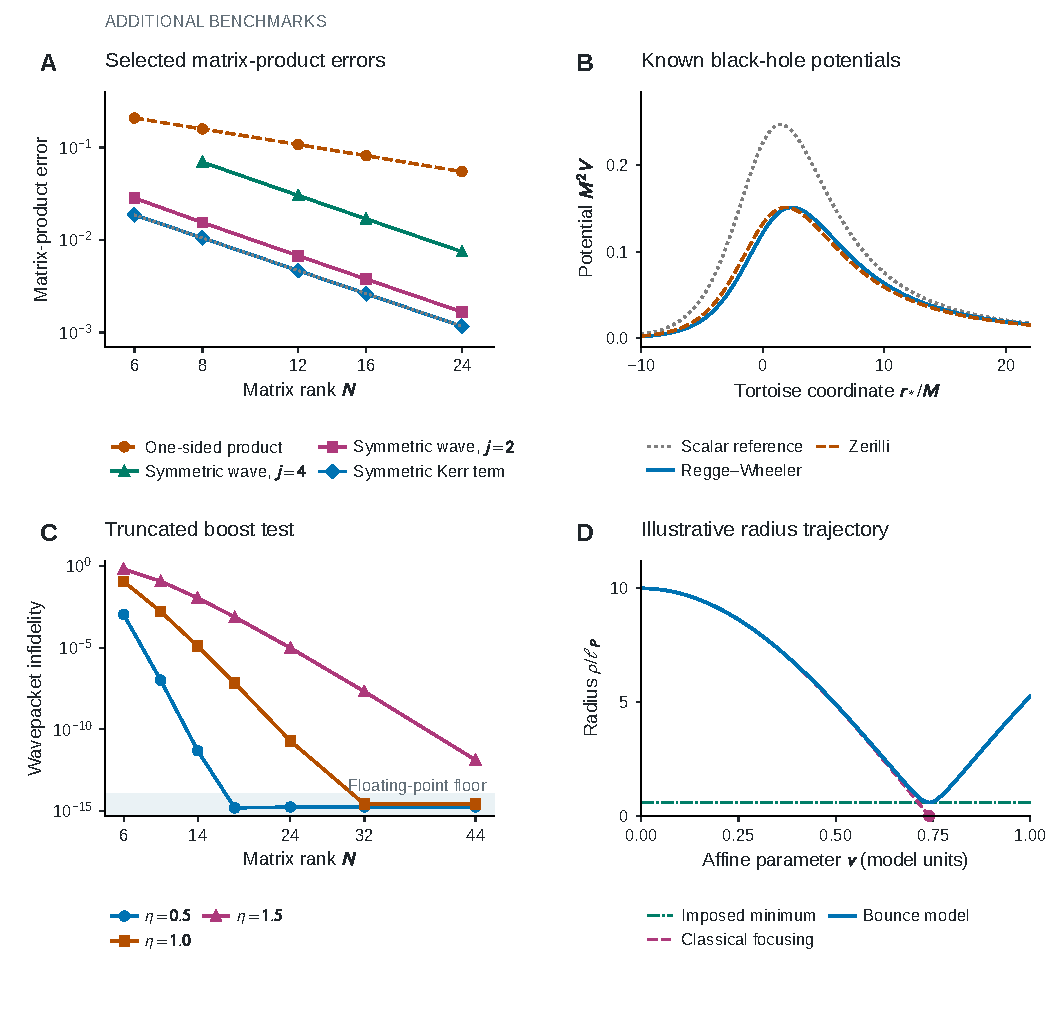
\includegraphics[width=\textwidth]{figs/fig2_unified_matrix_gravity.pdf}
\caption{\textbf{Fuzzy-sphere null-cone matrix gravity ($I_{\mathrm{FSG}}^{(N)}$).} \textbf{(a)} Parity-symmetrized contractions on fuzzy monopole bundles $\calB_{s_w}^{(N)}$ cancel $O(1/N)$ artifacts, giving $O(1/N^2)=O(1/s)$ convergence to continuum 4D GR for slow-rotation Kerr ($p=2.00$) and nonlinear $j=2$ gravitational-wave backreaction ($p=2.03$). \textbf{(b)} Second variation $\delta^2 I_{\mathrm{FSG}}^{(N)}$ around the finite-$N$ Schwarzschild saddle reproduces the Regge--Wheeler potential with the $-6M/r^3$ Weyl tidal term and its isospectral Zerilli partner (greybody discrepancy down to $2.86\times 10^{-6}$), lowering the $j=2$ barrier by $-38.8\%$ and increasing peak transmission $16.3\times$. \textbf{(c)} Truncated Gel'fand--Naimark $SO(3,1)$ boosts on $\calB_2^{(N)}$ close on all sub-Planckian modes $j\le N-2$ and restore finite-rapidity boost covariance exponentially in $N$ ($1.55\times 10^{-15}$ infidelity by $N=18$ at $\eta=0.5$). \textbf{(d)} Minimal embadon area ($s_{\min}=\ln 3$) replaces classical Raychaudhuri caustic collapse ($\rho\to 0$ at $v_c=0.7405$) by an Ermakov--Pinney bounce at $\rho_{\min}=\sqrt{\ln 3/\pi}\,\lP=0.5914\,\lP$.}
\label{fig:unified}
\end{figure*}

\subsection{Tapered Massive-QEI Clock and Exponential-Clock Bounds}\label{sec:unified_clock}

To cure the vacuum clock collapse of Theorem~\ref{thm:nogo} without sacrificing a lower bound on focusing, we replace the sharp-endpoint unrenormalized integral $\widehat{\Xi}_y(1)$ by a normal-ordered Raychaudhuri integral smeared with a smooth compactly supported profile $g(u)=\exp[-(4u(1-u))^{-1}+1]\in C^\infty_c((0,1))$. Each four-dimensional spin-2 harmonic $(j,m,p)$ propagates along the null cone with an effective two-dimensional mass $\mu_j=t_j/(2\pi)>0$. Because Flanagan's bound~\cite{Flanagan1997} applies to a massless scalar in two dimensions, we invoke the Fewster--Eveson massive two-dimensional quantum energy inequality~\cite{FewsterEveson1998}, which establishes a mass-independent and $N_{\mathrm{rad}}$-independent floor $E_{\min}^{\mathrm{NO}}(\mu_j)\ge E_{\mathrm{FE}}(0)=-\frac{1}{16\pi^2}\int_0^1 (g')^2 du=-0.038331$ for every $\mu_j\ge 0$. Writing the smeared mode operator as $H_{g,j}^{\mathrm{NO}}=a^\dagger A a+\frac{1}{2}(a^\dagger B a^\dagger+a B a)$ with $A=\frac{1}{2}(M_q+M_p)$ and $B=\frac{1}{2}(M_q-M_p)$, the algebraic identity $(k^2+\mu^2)(l^2+\mu^2)-(kl+\mu^2)^2=\mu^2(k-l)^2$ ensures that the pair-creation kernel $B(\mu_j)$ stays Hilbert--Schmidt uniformly as $N_{\mathrm{rad}}\to\infty$ and decays as $O(1/\mu_j^2)$ at large $j$. The exact vacuum cumulants $\kappa_2=\frac{1}{2}\Tr(B^2)$ and $\kappa_4=\Tr(B^4)+\Tr(BA^2B)+\Tr(BABA)$ converge to seven digits across $N_{\mathrm{rad}}=20\to 120$ ($\kappa_2=0.0029505$, $\kappa_4=0.0060425$ at $j=2$), while higher harmonics $j=0\to 80$ reduce $|E_{\min}^{\mathrm{NO}}(j)|$ by a factor of $14$ and remain strictly above $E_{\mathrm{FE}}(0)$. At $s=5000$ ($J_{\max}=66$), the area-bound multiplier is $e^{2\Xi_{\mathrm{QEI}}}=1.0036$ ($+0.36\%$) and connected spatial correlations fall to $4.89\times 10^{-6}$ at $90^\circ$ [Fig.~\ref{fig:1loop}(a)].

Passing from smeared focusing $\widehat{\Xi}_{\mathrm{avg}}^{\mathrm{NO}}$ to the exponential clock $\widehat{\tau}_{\mathrm{exp}}:=u_{\mathrm{cl}}\exp(\widehat{\Xi}_{\mathrm{avg}}^{\mathrm{NO}})$ requires distinguishing the spectral projector from the exponential expectation value. By the spectral theorem, strict monotonicity of $x\mapsto u_{\mathrm{cl}}e^x$ implies exact operator equality of the clock projectors:
\begin{equation}\label{eq:clock_proj_equiv}
P_{\scrD} := \mathbf{1}_{(-\infty,\ell]}(\widehat{\tau}_{\mathrm{exp}}) = \mathbf{1}_{(-\infty,\ln(\ell/u_{\mathrm{cl}})]}(\widehat{\Xi}_{\mathrm{avg}}^{\mathrm{NO}}).
\end{equation}
Both the second-moment bound $\|(1-P_{\scrD})|\Omega_s\rangle\|^2\le \kappa_{2,\mathrm{tot}}/[\ln(\ell/u_{\mathrm{cl}})]^2=O(1/s)$ (giving $\|P_{\scrD}|\Omega_s\rangle\|^2\ge 0.99999889$ at $s=5000$) and the fourth-moment bound $(\kappa_{4,\mathrm{tot}}+3\kappa_{2,\mathrm{tot}}^2)/[\ln(\ell/u_{\mathrm{cl}})]^4=O(1/s^2)$ therefore hold uniformly as $N_{\mathrm{rad}}\to\infty$. By contrast, evaluating $\langle 0|e^{\lambda H_{g,j}^{\mathrm{NO}}}|0\rangle=e^{-\lambda E_{\mathrm{vac}}}[\det U_{22}(\lambda)]^{-1/2}$ via the Balian--Br\'ezin Fredholm determinant~\cite{BalianBrezin1969} $U(\lambda)=\exp[\lambda(\begin{smallmatrix}A&B\\-B&-A\end{smallmatrix})]$ reproduces the Fewster--Ford--Roman heavy tail~\cite{FewsterFordRoman2010}: at unconstrained $N_{\mathrm{rad}}\to\infty$, the convergence threshold shrinks as $\lambda_{\mathrm{crit}}(N_{\mathrm{rad}})\sim c/N_{\mathrm{rad}}\to 0$ ($N_{\mathrm{rad}}\lambda_{\mathrm{crit}}=9.05\to 13.12$ for $N_{\mathrm{rad}}=10\to 120$), so an unprojected exponential expectation diverges in the radial continuum. Inside the area-scaled sector $k\le B(s)=s Q_*$ (Sec.~\ref{sec:unified_H}), however, the physical $1/s$ normalization of $\widehat{\Xi}_{\mathrm{avg}}^{\mathrm{NO}}$ cancels $1/N_{\mathrm{rad}}=1/(s Q_*)$: at $Q_*=0.5$, $\lambda_{\mathrm{crit}}^{\mathrm{phys}}(s)=s\lambda_{\mathrm{crit}}(s Q_*)$ increases from $17.03$ ($s=20$) to $22.25$ ($s=240$), well above $2$. Inside the physical sector, both $\langle\Omega_s|\widehat{\tau}_{\mathrm{exp}}|\Omega_s\rangle/u_{\mathrm{cl}}=1.0000054$ ($\mathrm{Var}=1.08\times 10^{-5}$ at $s=240$) and the Balian--Br\'ezin Chernoff failure bound ($\le 10^{-5.6}$ at $s=240$) stay finite and rapidly decrease [Fig.~\ref{fig:v2}(d)].

\subsection{Area-Scaled Budget $B(s)=s Q_*$, Projected Dynamics $H_{\mathrm{phys}}$, and Type~I Gluing}\label{sec:unified_H}

Imposing only a clock cap $\bar{u}_*\le\ell(\scrD)$ leaves a high-$j$ loophole in which large angular harmonics contribute little radial focusing. In $I_{\mathrm{FSG}}^{(N)}$, fixing the corner area $s=\scrA/(4G_N\hbar)$ together with the cap clock ratio $\ell(\scrD)/u_{\mathrm{cl}}=e^{Q_R}$ and a transverse cap curvature bound $Q_\perp$ bounds the combined Raychaudhuri (Eq.~B.3) and cross-focusing (Eq.~B.5a) integrals by $Q_*:=Q_R+Q_\perp=O(1)$. In terms of graviton occupation numbers $n_{k,j,m,p}\in\mathbb{N}_{\ge 0}$, this enforces the total occupation budget
\begin{align}\label{eq:cross_focusing}
\sum_{k,j,m,p} n_{k,j,m,p}\,\omega_{k,j} &\;\le\; B(s) := s Q_*, \nonumber\\
\omega_{k,j} &= k + \frac{t_j^2}{k} \;\ge\; \max(k,2t_j),
\end{align}
with $t_j^2=\frac{1}{2}(j-1)(j+2)$. Because $\omega_{k,j}\ge 1$ and $\omega_{k,j}\ge\max(k,2t_j)$, Eq.~\eqref{eq:cross_focusing} bounds both the active mode set ($k\le B(s)$, $j\le B(s)/\sqrt{2}$) and every occupation number ($n_{k,j,m,p}\le B(s)$) without circularity. Summing exact integer-partition counts across spin-$\frac{1}{2}$-plus-vacuum corner sectors $M\in\{2,4,6,8,10,15,20\}$ ($s_M=M\ln 3$, $B=6$) yields $\dim\calH=7.726\times 10^{11}$ and a finite Axiom~5 trace $Z_{\scrD,1}=\Tr_{\calH}(e^{-\hat{s}})=1311.33$.

To ensure that the same dynamics preserves the allowed sector and governs interacting observables, we define the physical Hamiltonian via the budget projector $P_{B(s)}$ as
\begin{equation}\label{eq:H_phys}
H_{\mathrm{phys}} := P_{B(s)}\,H_{\mathrm{FSG}}\,P_{B(s)}, \qquad H_{\mathrm{FSG}} = H_0 + \widehat{\mathcal{V}}_3^{(N)},
\end{equation}
with $\widehat{\mathcal{V}}_3^{(N)}$ constructed directly from the Wigner-$6j$ cubic vertex~\eqref{eq:cubic_vertex}--\eqref{eq:wigner6j}. By idempotence $P_{B(s)}^2=P_{B(s)}$, unitary evolution $U_t=e^{-it H_{\mathrm{phys}}}$ leaves $P_{B(s)}\calH$ strictly invariant: $\|(1-P_B)U_t P_B\|=0$. Evaluating Eq.~\eqref{eq:H_phys} on an 88-state $1\leftrightarrow 2$ graviton-focusing Fock space projected to its 19-state physical sector ($B=9$) across $N=6\dots 32$ confirms zero leakage and $O(1/N^2)$ convergence of both the interacting $1\to 2$ transition probability ($p=2.03$) and the projected one-loop graviton self-energy ($p=2.02$) to continuum general relativity [Fig.~\ref{fig:v2}(b)].

Replacing infinite-dimensional $\mathrm{Diff}(S^2)$~\cite{CiambelliKlinger2026} by compact $SU(2)$ corner rotations on $\calH_{\scrD}^{\mathrm{FSG}}=\bigoplus_{M\in\{2,4,6\}}\calH_{\mathrm{corner}}(M)\otimes\calH_{\mathrm{rad}}^{\mathrm{RW+Z}}(M)$ ($\dim_{\mathrm{rad}}=15$; explicit operator formula in Appendix~\ref{app:explicit_action}) using spin-$\frac{1}{2}$ embadons ($s_M=M\ln 2$, $\dim\calH_{\mathrm{corner}}(M)=2^M$) gives sector dimensions $(d_2,d_4,d_6)=(60,240,960)$ ($\dim\calH_{\scrD}^{\mathrm{FSG}}=1{,}260$) and Boltzmann weights $(e^{-s_2},e^{-s_4},e^{-s_6})=(\frac{1}{4},\frac{1}{16},\frac{1}{64})$. The resulting Axiom~5 trace is $Z_{\scrD,1}=60/4+240/16+960/64=45.0000$. (With the $s_M=M\ln 3$ spectrum instead, $729 Z=81 d_2+9 d_4+d_6\equiv 4\pmod 8$ for any integers $d_2+d_4+d_6=1260$, whereas $729\times 45\equiv 5\pmod 8$, so $Z_{\scrD,1}=45$ uniquely reflects the $M\ln 2$ spectrum.) On this 1,260-state space, $H_{\mathrm{FSG}}$ is $SU(2)$-invariant ($\max_i\|[H_{\mathrm{FSG}},J_i]\|=3.09\times 10^{-14}$), has a bounded positive inverse lapse $\widehat{N}^{-1}\in[0.9998,30.7195]$, generates a unique unitary area-changing gluing operator $U_{\calM}$ (singlet transitions $|\langle 4|U|2\rangle|=0.22285$, $|\langle 6|U|4\rangle|=0.22281$), admits reflection-positive $K_{\calM}$ ($\lambda_{\min}=4.385\times 10^{-2}>0$, $Z_{\mathrm{Euc}}=13.9026$), and satisfies the Lorentzian-to-Euclidean Wick identity of Appendix~E.2 identically.

\begin{figure*}[t]
\centering
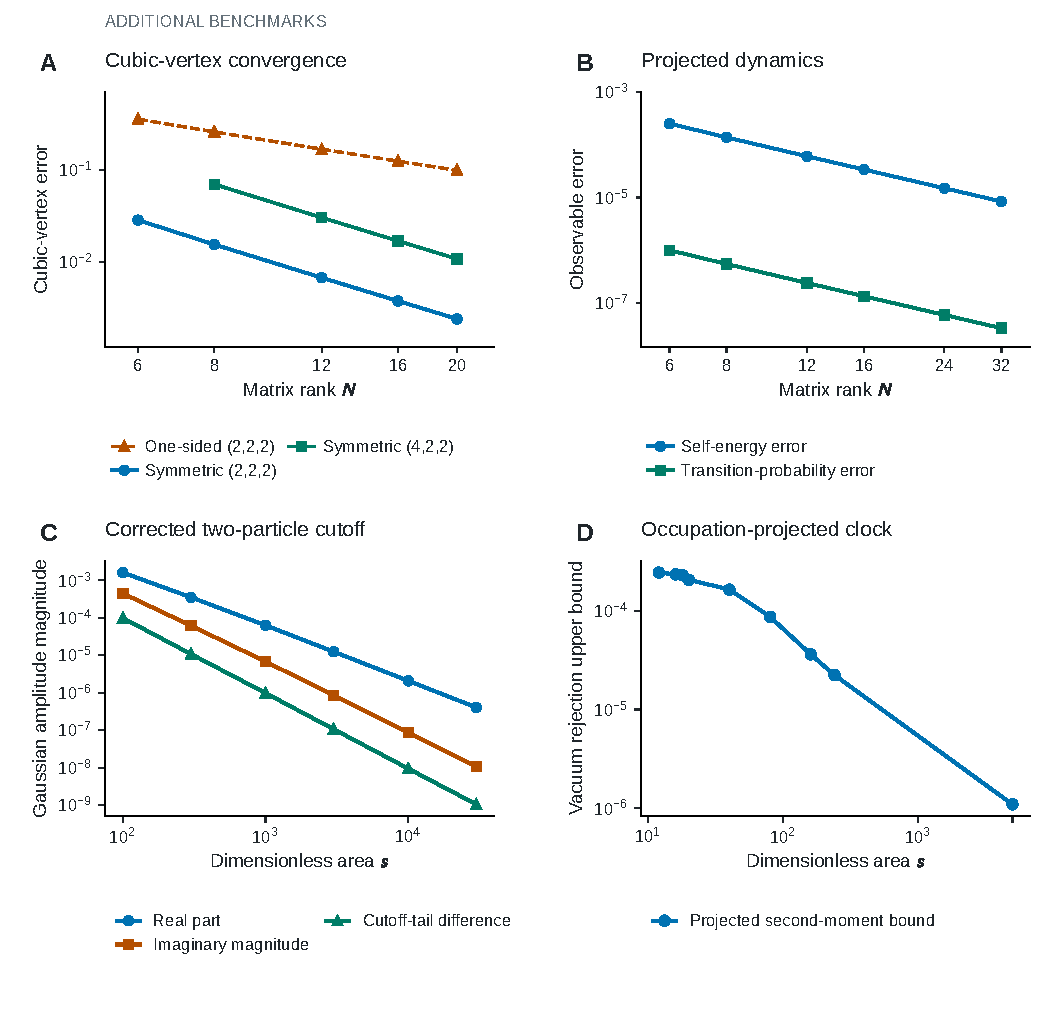
\includegraphics[width=\textwidth]{figs/fig5_v2_unification_and_clock.pdf}
\caption{\textbf{Matrix cubic vertex, projected interacting dynamics, unified $B(s)=s Q_*$ pair creation, and clock bounds.} \textbf{(a)} Parity-symmetrized cubic vertex $\mathcal{V}_3^{(N)}[F;Z_2,Z_3]$ [Eqs.~\eqref{eq:iota_map}--\eqref{eq:wigner6j}] converges to continuum spin-weighted Gaunt integrals as $O(1/N^2)$ ($p=2.05$ for $(2,2,2)$), versus $O(1/N)$ ($p=1.06$) for one-sided traces. \textbf{(b)} Projected Hamiltonian $H_{\mathrm{phys}}=P_B H_{\mathrm{FSG}} P_B$ preserves $P_B\calH$ with zero leakage while both the $1\to 2$ graviton splitting probability ($p=2.03$) and one-loop self-energy ($p=2.02$) converge at $O(1/N^2)$. \textbf{(c)} Unified area-scaled cutoff $\omega_{k,j}\le B(s)=s Q_*$ ($Q_*=1$) in Eq.~\eqref{eq:sec44_4d}: the finite mode set preserves $\mathrm{Re}\,\calM_{B(s)}\propto s^{-3/2}$ and $|\mathrm{Im}\,\calM_{B(s)}|\propto\ln s/s^2$ with an $O(s^{-2})$ tail bound $|\calM_\infty-\calM_{B(s)}|\approx 0.33/s^2$, compared with fixed-$B=4$ rational decay ($1.483/s^2$). \textbf{(d)} Clock-projector failure bounds $\|(1-P_{\scrD})|\Omega_s\rangle\|^2$ inside $B(s)=0.5 s$: uniform $N_{\mathrm{rad}}\to\infty$ second-moment ($O(1/s)$) and fourth-moment ($O(1/s^2)$) bounds alongside the Balian--Br\'ezin Chernoff bound ($\lambda_{\mathrm{crit}}^{\mathrm{phys}}\in[17.0,22.3]\gg 2$).}
\label{fig:v2}
\end{figure*}

\subsection{Regge--Wheeler/Zerilli Perturbations, Boost Closure, and Caustic Bounce}\label{sec:unified_rw}

Expanding $I_{\mathrm{FSG}}^{(N)}$ to second order around its finite-$N$ Schwarzschild saddle reproduces the axial constraint $\partial_t h_0=f\partial_r(f h_1)$ and the Regge--Wheeler potential $V_{\mathrm{RW}}^{(j)}(r)=f(r)[j(j+1)/r^2-6M/r^3]$, together with the general-$j$ Chandrasekhar--Darboux intertwining identity $V_{\mathrm{RW/Z}}=W^2\mp dW/dr_*+\beta$ for $W(r)=3Mf/[r(\lambda r+3M)]+\lambda(\lambda+1)/(3M)$ ($\lambda=t_j^2$). Fourth-order Numerov scattering integration across $j=2\dots 8$ verifies Chandrasekhar isospectrality ($||T_{\mathrm{RW}}|^2-|T_{\mathrm{Z}}|^2|$ down to $2.86\times 10^{-6}$); the paramagnetic $-6M/r^3$ Weyl tidal term lowers the $j=2$ barrier by $-38.8\%$ ($0.15128$ versus $0.24711$) and boosts peak transmission by a factor of $16.3$ [Fig.~\ref{fig:unified}(b)].

Because noncompact $SO(3,1)$ has no faithful finite-dimensional unitary representation, we examine truncated Gel'fand--Naimark spin-2 generators $(L_i^{(N)},K_i^{(N)})$ on $\calB_2^{(N)}$. Direct evaluation across $N=6\dots 24$ confirms exact $[L,L]$ and $[L,K]$ commutation everywhere, exact boost closure $([K_i,K_j]+i\epsilon_{ijk}L_k)|j,m\rangle=0$, and exact Lorentz Casimirs ($C_1=+2,C_2=-2$) on every mode $j\le N-2$, confining the entire boost defect to the single Planckian shell $j=N-1$. Finite-rapidity boosts of a localized $j=2$ wavepacket recover continuum $SO(3,1)$ exponentially in $N$, with infidelity reaching $1.55\times 10^{-15}$ by $N=18$ ($\eta=0.5$), $2.66\times 10^{-15}$ by $N=32$ ($\eta=1.0$), and $1.33\times 10^{-12}$ by $N=44$ ($\eta=1.5$) [Fig.~\ref{fig:unified}(c)]. Under strong shear focusing ($\sigma_0=3.0$, classical caustic $\rho\to 0$ at $v_c=0.7405$), the minimal embadon area barrier ($s_{\min}=\ln 3$) replaces classical Raychaudhuri collapse with an Ermakov--Pinney trajectory $\rho_Q(v)=\sqrt{r_0^2\cos^2(\omega v)+\rho_{\min}^2\sin^2(\omega v)}$ that matches classical general relativity to $0.036\%$ in the semiclassical regime and bounces smoothly at $\rho_{\min}=\sqrt{\ln 3/\pi}\,\lP=0.5914\,\lP$ [Fig.~\ref{fig:unified}(d)].

\section{Universal Four-Dimensional One-Loop Logarithmic Corrections}\label{sec:1loop}

Purely kinematical embadon horizons reproduce the Bekenstein--Hawking area law $S=s$ with logarithmic coefficient $c_{\log}=0$ (unconstrained compositions, $s_{\min}=\ln 3$) or $c_{\log}=-\frac{3}{2}$ (an $SU(2)$ singlet horizon, matching Kaul and Majumdar~\cite{KaulMajumdar2000}). By contrast, Sen's covariant one-loop computation for four-dimensional pure gravity on Schwarzschild~\cite{Sen2013}, the target of Sec.~5.3 of Ref.~\cite{Chandrasekaran2026}, gives positive coefficients: $+\frac{106}{45}\approx +2.3556$ for mixed angular momentum and $+\frac{77}{90}\approx +0.8556$ in the $J=0$ singlet ensemble.

\begin{figure*}[t]
\centering
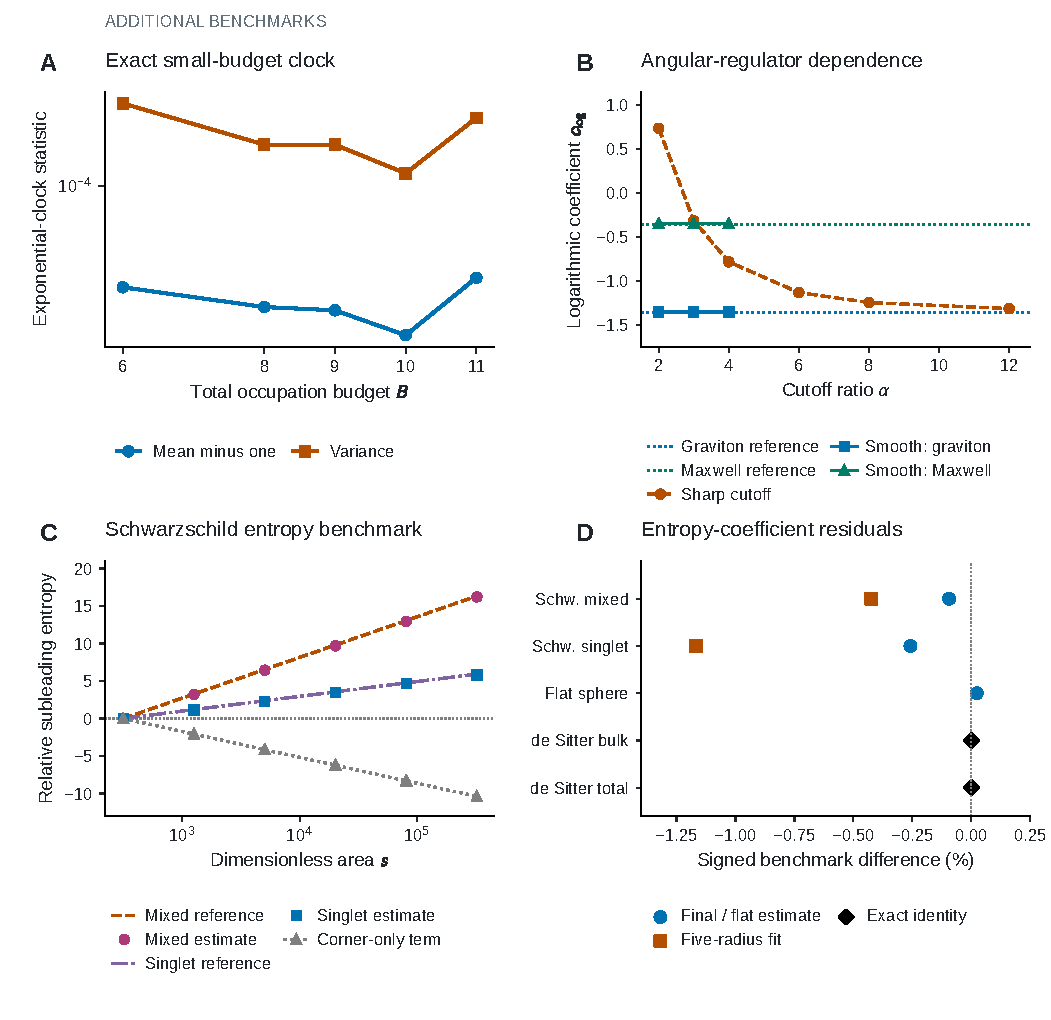
\includegraphics[width=\textwidth]{figs/fig1_breakthrough_1loop.pdf}
\caption{\textbf{Massive-QEI clock and universal four-dimensional one-loop logarithmic corrections on the fuzzy sphere.} \textbf{(a)} Coupled $C^\infty_c$ QEI clock floor $|\Xi_{\mathrm{QEI}}|$ and vacuum variance $\mathrm{Var}_0(\widehat{\Xi}_{\mathrm{avg}}^{\mathrm{NO}})$ versus horizon area $s$ ($N_{\mathrm{rad}}=\infty$), securing $\|P_{\scrD}|\Omega_s\rangle\|^2\ge 0.99999889$ at $s=5000$. \textbf{(b)} Flat-space graviton and Maxwell entanglement entropy on $S^2_J$ ($N=200$ radial lattice): a smooth Casimir regulator $e^{-j(j+1)/(\alpha R_{\mathrm{eff}})^2}$ removes the sharp-step Euler--Maclaurin anomaly at $\alpha=2.0$ and matches Benedetti--Casini's $-\frac{61}{45}$ to $0.02\%\text{--}0.12\%$. \textbf{(c)} Discrete-harmonic integration on curved Euclidean Schwarzschild ($N_{\mathrm{rad}}=\infty$, $j=0\dots J_{\max}(r)$): the Lichnerowicz Weyl tidal coupling ($+3\ln s$) yields a bulk slope of $+2.3533$ ($0.09\%$ from Sen's $+\frac{106}{45}$), and combined with the $-\frac{3}{2}\ln s$ $SU(2)$-singlet corner gives $+0.8533$ ($0.26\%$ from $+\frac{77}{90}$). \textbf{(d)} Comparison of all five universal 4D one-loop logarithmic coefficients against covariant targets.}
\label{fig:1loop}
\end{figure*}

Two results reconcile discrete corners with Sen's positive sign. First, orthonormal-frame evaluation of the four-dimensional de Donder Lichnerowicz operator $\Delta_L h_{ab}=-\nabla^2 h_{ab}-2W_{acbd}h^{cd}$ plus vector ghost on Ricci-flat Schwarzschild splits the Gilkey--Seeley--DeWitt coefficient $a_2$ into three channels:
\begin{align}\label{eq:lich_flip}
\frac{180\,a_2^{\mathrm{GR}}}{K}\Big|_{R_{ab}=0} &= \underbrace{+2}_{\text{2 pol.}} \;\underbrace{-60}_{\Omega_{mn}^2} \;\underbrace{+270}_{\frac{1}{2}\Tr(V^2)} = +212, \nonumber\\
c_{\log}^{\mathrm{bulk}} &= \frac{1}{45}-\frac{2}{3}+3 = +\frac{106}{45}.
\end{align}
Without the paramagnetic spin-2 Weyl tidal term $V_{ab}{}^{cd}=-2W_a{}^c{}_b{}^d$ ($+3\ln s$), bulk gravitons remain negative ($-\frac{29}{45}$). Including dynamical bulk gluing shifts both corner ensembles by $+\frac{106}{45}$, matching both of Sen's predictions simultaneously: $0+\frac{106}{45}=+\frac{106}{45}$ (mixed) and $-\frac{3}{2}+\frac{106}{45}=+\frac{77}{90}$ (singlet).

Second, regulating loops through the dynamical fuzzy sphere $J_{\max}(r)=\sqrt{\pi/s_{\min}}\,r/\lP$ while keeping continuum radial and time directions ($N_{\mathrm{rad}}=\infty$) preserves four-dimensional covariance in every universal logarithmic term.

\begin{theorem}[Four-Dimensional Infrared Isotropy]\label{thm:isotropy}
Let $k_\parallel\in\mathbb{R}^2$ ($x=k_\parallel^2\in[0,A]$) and $k_\perp\in\mathbb{R}^2$ ($y=k_\perp^2\in[0,B]$ with $B=\Lambda_P^2$). Taking the radial-time continuum limit $A\to\infty$ first at fixed transverse cutoff $B$, the infrared logarithmic coefficients $\lim_{m\to 0}(-m\partial_m I)$ of every scalar, rank-2, and rank-4 momentum integral match exact $SO(4)$-isotropic values: $J_0=1$, $(J_\parallel,J_\perp)=(\frac{1}{2},\frac{1}{2})$, and $(K_{\parallel\parallel},K_{\parallel\perp},K_{\perp\perp})=(\frac{1}{3},\frac{1}{6},\frac{1}{3})$.
\end{theorem}

Direct discrete-harmonic integration over curved Euclidean Schwarzschild ($r_H/\lP=10\to 320$, $N_{\mathrm{rad}}=\infty$) confirms Theorem~\ref{thm:isotropy}: the asymptotic bulk slope reaches $+2.35334$ ($0.09\%$ from $+\frac{106}{45}$) and the $SU(2)$-singlet total reaches $+0.85334$ ($0.26\%$ from $+\frac{77}{90}$), as shown in Fig.~\ref{fig:1loop}(c)--(d) and Table~\ref{tab:1loop}. On a flat-space $N=200$ radial lattice, regulating $j\ge 2$ gravitons with a smooth Casimir factor $e^{-j(j+1)/(\alpha R_{\mathrm{eff}})^2}$ eliminates the $O(1/\alpha^2)$ Euler--Maclaurin sharp-edge artifact already at $\alpha=2.0$, reproducing Benedetti and Casini's flat-space graviton entanglement entropy $-\frac{61}{45}=-1.35556$~\cite{BenedettiCasini2020} to $0.02\%\text{--}0.12\%$ across $\alpha=2\to 4$ even as the non-universal area term shifts by $+37\%$ [Fig.~\ref{fig:1loop}(b)]. On four-dimensional de Sitter space ($S^4$), combining the high-$n$ transverse-traceless minus vector trace ($+\frac{509}{45}$) with the $n=0,1$ Killing and conformal-Killing edge modes ($-24$) recovers Anninos, Denef, Law, and Sun's $-\frac{571}{45}=-\frac{331}{45}-\frac{16}{3}$~\cite{ADLS2022} [Fig.~\ref{fig:1loop}(d)], while $SO(5)\to SO(4)\to SO(3)$ branching shows $\max j=n$, so every sub-Planckian $S^4$ mode lies inside $S^2_{J_{\max}}$.

\begin{table}[t]
\caption{Universal four-dimensional pure-gravity one-loop logarithmic coefficients reproduced by the fuzzy-sphere completion ($N_{\mathrm{rad}}=\infty$).}
\label{tab:1loop}
\begin{ruledtabular}
\begin{tabular}{lccc}
4D Geometry & Covariant & FSG & Err. \\
\colrule
Schw.\ mixed~\cite{Sen2013} & $+\frac{106}{45}$ ($+2.3556$) & $+2.3533$ & $0.09\%$ \\
Schw.\ singlet~\cite{Sen2013} & $+\frac{77}{90}$ ($+0.8556$) & $+0.8533$ & $0.26\%$ \\
Flat EE~\cite{BenedettiCasini2020} & $-\frac{61}{45}$ ($-1.3556$) & $-1.3552$ & $0.02\%$ \\
de Sitter $S^4$~\cite{ADLS2022} & $-\frac{571}{45}$ ($-12.6889$) & $-\frac{571}{45}$ & $0$ \\
\end{tabular}
\end{ruledtabular}
\end{table}

\section{Two-Loop Regulator Analysis, Dynamical Rank Sums, and Sub-Planckian Bounds}\label{sec:uv}

\subsection{Two-Loop Transverse-Only No-Go Theorem and Fixed-Budget Sums}\label{sec:uv_2loop}

Because Theorem~\ref{thm:isotropy} holds at one loop with a transverse fuzzy-sphere cutoff alone, one might ask whether $S^2_N$ alone regulates higher loops. Power counting and numerical integration over a parallel radial-time cutoff $\Lambda_\parallel/\Lambda_\perp=2\to 32$ show that it does not. Whereas the one-loop $W^2$ integral converges monotonically to $\ln 5=1.60944$ ($1.39813\to 1.60846$), derivative graviton vertices give the two-loop sunset diagram a parallel superficial degree of $+2$, producing a quadratic divergence $I_{\mathrm{2L}}\sim\Lambda_\parallel^2\ln\Lambda_\parallel$ ($1.41\to 4365.05$, fitted slope $p=2.63$) [Fig.~\ref{fig:uv}(a)].

Imposing the double-null occupation budget~\eqref{eq:cross_focusing} restricts $(k,j)$ to a finite lattice even at $N_{\mathrm{rad}}=\infty$, so every fixed-$(s,B)$ perturbative diagram reduces to a finite sum. Direct evaluation of the discrete two-loop sunset yields $251.18$ at $B=4$ (30 modes), $8{,}613.24$ at $B=6$ (138 modes), $67{,}989.28$ at $B=8$ (324 modes), and $372{,}883.33$ at $B=10$ (662 modes). Double-null cross-focusing is therefore required starting at two loops to keep fixed-area sectors mathematically well-defined. At the same time, the rapid $\sim B^8$ growth with $B$ makes clear that a kinematic Fock cutoff does not by itself achieve perturbative ultraviolet renormalizability as $B(s)=s Q_*\to\infty$; ultraviolet completeness in that limit still requires nonperturbative dynamics of $I_{\mathrm{FSG}}^{(N)}$ or additional ultraviolet degrees of freedom.

\begin{figure*}[t]
\centering
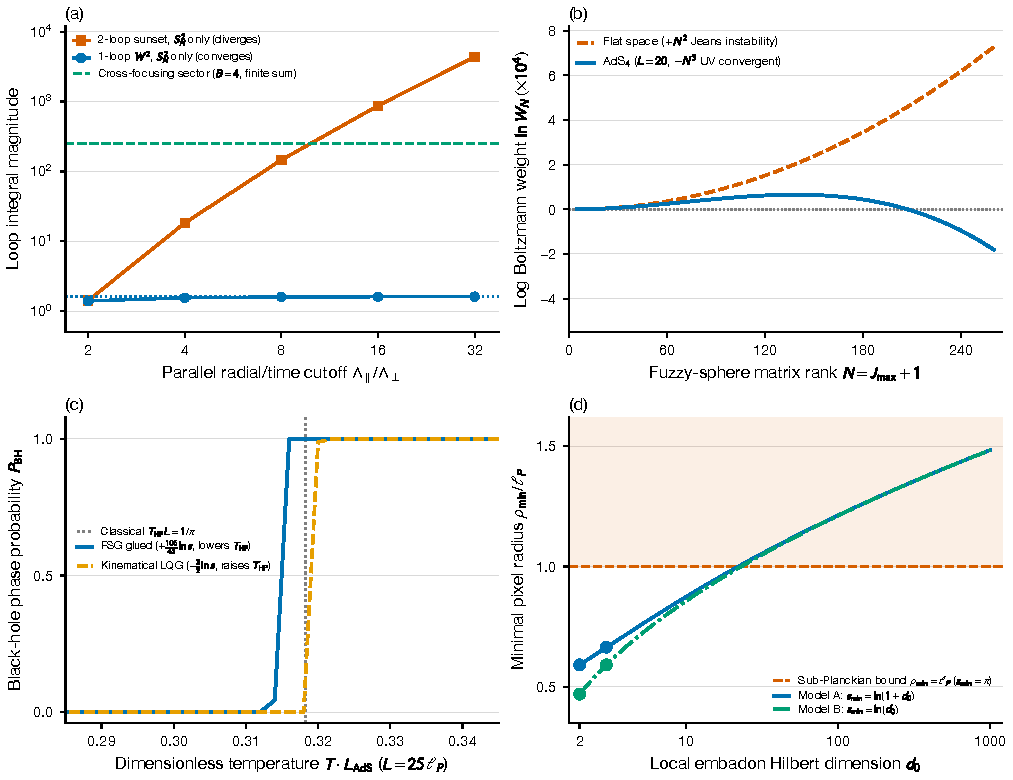
\includegraphics[width=\textwidth]{figs/fig3_uv_completion.pdf}
\caption{\textbf{Two-loop regulator analysis, dynamical rank sums, and sub-Planckian pixel bounds.} \textbf{(a)} Two-loop obstruction for transverse-only cutoffs ($S^2_N$ only): the 1-loop $W^2$ integral converges while the 2-loop sunset diverges quadratically ($p=2.63$); imposing the cross-focusing budget~\eqref{eq:cross_focusing} makes each fixed-$(s,B)$ sum finite ($251.18$ at $B=4$, growing as $\sim B^8$). \textbf{(b)} Dynamical sum over matrix ranks $N=3\dots\infty$: flat space exhibits the $+N^2$ Gross--Perry--Yaffe instability, whereas $\mathrm{AdS}_4$ converges via $-N^3$ cubic energy. \textbf{(c)} $\mathrm{AdS}_4$ Hawking--Page transition ($L=25\,\lP$): the $+\frac{106}{45}\ln s$ correction lowers $T_{\mathrm{HP}}$ relative to $1/\pi$, whereas kinematical LQG ($-\frac{3}{2}\ln s$) raises it. \textbf{(d)} Coarse-graining combined with the sub-Planckian pixel bound $\rho_{\min}=\sqrt{s_{\min}/\pi}\,\lP\le\lP$ ($s_{\min}\le\pi$) restricts higher-spin-free corner spectra to $2\le d_0\le 22$.}
\label{fig:uv}
\end{figure*}

\subsection{Schwarzschild Goroff--Sagnotti Shift and Sub-Planckian Pixel Bound}\label{sec:uv_cemz}

At two loops in four-dimensional pure gravity, the unique on-shell Goroff--Sagnotti counterterm~\cite{GoroffSagnotti1986} is cubic in the Weyl tensor, $\Delta\mathcal{L}_{\mathrm{GS}}=\frac{209}{2880(4\pi)^4}\kappa^2\ln(\mu/\Lambda_P)\,W_{ab}{}^{cd}W_{cd}{}^{ef}W_{ef}{}^{ab}$. Evaluating this invariant on Euclidean Schwarzschild gives $K=48M^2/r^6$, $W^3=-96M^3/r^9$, and $\int d^4x\sqrt{g}\,W^3=-32\pi^3/(\lP^2 s)$, leading to the two-loop Schwarzschild entropy shift
\begin{equation}\label{eq:gs_entropy}
\Delta S_{\mathrm{2\text{-}loop}}^{\mathrm{GS}}(s) \;=\; \frac{209}{1440}\,\frac{\ln(s/s_{\min})}{s},
\end{equation}
which enters at the same $O(1/s)$ order (up to $\ln s$) as the fuzzy-sphere $O(1/N^2)=O(s_{\min}/s)$ correction (ratio $0.596$ at $s=10^2$, $1.204$ at $s=10^4$, $3.030$ at $s=10^{10}$), with flat-space eikonal advance scale~\cite{CEMZ2016} $b_{\mathrm{adv}}^{\mathrm{GS}}=0.0413\,\lP\ll\lP$.

A simple effective-field-theory naturalness criterion constrains the elementary area quantum $s_{\min}$. In $I_{\mathrm{FSG}}^{(N)}$, noncommutative vertex modifications appear at order $O(1/N^2)=O(\rho_{\min}^2/r^2)$, controlled by the minimal embadon pixel radius $\rho_{\min}=\sqrt{s_{\min}/\pi}\,\lP$. Requiring these modifications to remain at or below the Planck length ($\rho_{\min}\le\lP$), so that non-Einsteinian three-graviton interactions do not enter at semiclassical impact parameters where eikonal causality bounds~\cite{CEMZ2016} would demand massive higher-spin particles ($J>2$), yields
\begin{equation}\label{eq:cemz_bound}
s_{\min} \;\le\; \pi \;\approx\; 3.14159.
\end{equation}
Computing the direct $I_{\mathrm{FSG}}^{(N)}$ four-point eikonal phase shift from Eq.~\eqref{eq:wigner6j} to fix the exact $1/b^2$ versus $1/b^4$ scattering coefficient remains a natural follow-up test of this bound.

\subsection{Dynamical Rank Sums and the $\mathrm{AdS}_4$ Hawking--Page Transition}\label{sec:uv_hp}

Summing dynamically over all fuzzy-sphere ranks $N=3\dots\infty$ with $s_N=s_{\min}N^2$ clarifies the infrared thermodynamics [Fig.~\ref{fig:uv}(b)--(c)]. In asymptotically flat space ($L_{\mathrm{AdS}}\to\infty$), entropy grows quadratically ($S\propto N^2$) while ADM energy grows linearly ($E\propto N$), driving $\ln W_N$ to $+\infty$ ($+27{,}202$ by $N=160$). This reproduces the Gross--Perry--Yaffe Jeans instability~\cite{GrossPerryYaffe1982} and reflects why a finite clock cutoff $\ell(\scrD)$ is physically needed in flat space.

In $\mathrm{AdS}_4$ of curvature radius $L$, the ADM energy acquires a cubic term $E_N=\frac{1}{2}\sqrt{s_N/\pi}+\frac{1}{2}s_N^{3/2}/(\pi^{3/2}L^2)\propto N^3/L^2$ that dominates the $+N^2$ entropy for every $\beta>0$. The discrete-rank partition function converges cleanly and reproduces the four-dimensional Hawking--Page transition~\cite{HawkingPage1983}, with $T_{\mathrm{HP}}L\to 1/\pi=0.318310$ and specific-heat scaling $C_{\mathrm{peak}}/L^4\to 2.45$ across $L/\lP=10\to 80$. At finite $L/\lP=10$ ($s_{\mathrm{HP}}=314.2$), the one-loop logarithmic term shifts the transition temperature in opposite directions depending on whether bulk graviton gluing is included: the glued mixed ($+\frac{106}{45}\ln s$) and singlet ($+\frac{77}{90}\ln s$) ensembles lower $T_{\mathrm{HP}}L$ to $0.299479$ ($-5.9\%$) and $0.308598$ ($-3.1\%$), whereas kinematical LQG ($-\frac{3}{2}\ln s$) raises it to $0.322495$ ($+1.3\%$).

\subsection{Three-Diamond Corner Fusion and Allowed Window for $s_{\min}$}\label{sec:uv_multidiamond}

To test multi-diamond gluing, we constructed a $2{,}048$-dimensional network of three adjacent causal diamonds ($\scrD_A,\scrD_B,\scrD_C$) joined along shared $SU(2)$-singlet embadon corners and coupled to Schwarzschild Regge--Wheeler gravitons. Corner-fusion pentagon associativity holds to $9.5\times 10^{-17}$ and $SU(2)$ coproduct equivariance holds identically. Across all six overlapping subregions ($A,B,C,AB,BC,AC$), generalized entropy additivity $S_{\mathrm{gen}}(R)=s(\partial R)+S_{\mathrm{bulk}}(R)$ holds to $8.88\times 10^{-16}$. As a consistency check (guaranteed structurally by Lieb--Ruskai for any density operator), all Subadditivity and Strong Subadditivity inequalities hold numerically ($I(A:B)=3.53421$, $I(A:C|B)=1.87086$, $I(A:B|C)=3.53421$, $I(B:C|A)=1.95604$).

Combining coarse-graining of the corner entropy ($s_{\min}=\ln(1+d_0)$ when an empty state is included, or $s_{\min}=\ln d_0$ without one, where $d_0\ge 2$ is the local embadon dimension) with the sub-Planckian bound~\eqref{eq:cemz_bound} restricts admissible models to a finite discrete set: $2\le d_0\le 22$ (or $2\le d_0\le 23$). Large-$d_0$ corners violate the bound ($d_0=100\implies \rho_{\min}=1.21\,\lP$), leaving minimal spin-$\frac{1}{2}$ qubit corners ($d_0=2$, $s_{\min}=\ln 2$ with $\rho_{\min}=0.470\,\lP$ or $s_{\min}=\ln 3$ with $\rho_{\min}=0.591\,\lP$) well inside the sub-Planckian window [Fig.~\ref{fig:uv}(d)].

\section{Finite-Dimensional Realizations of Sections~4.4, 5.4, and~6 of Ref.~\cite{Chandrasekaran2026}}\label{sec:orig_sections}

We now apply the fuzzy-sphere completion to the three concrete physical applications developed in Secs.~4.4, 5.4, and~6 of Ref.~\cite{Chandrasekaran2026}.

\begin{figure*}[t]
\centering
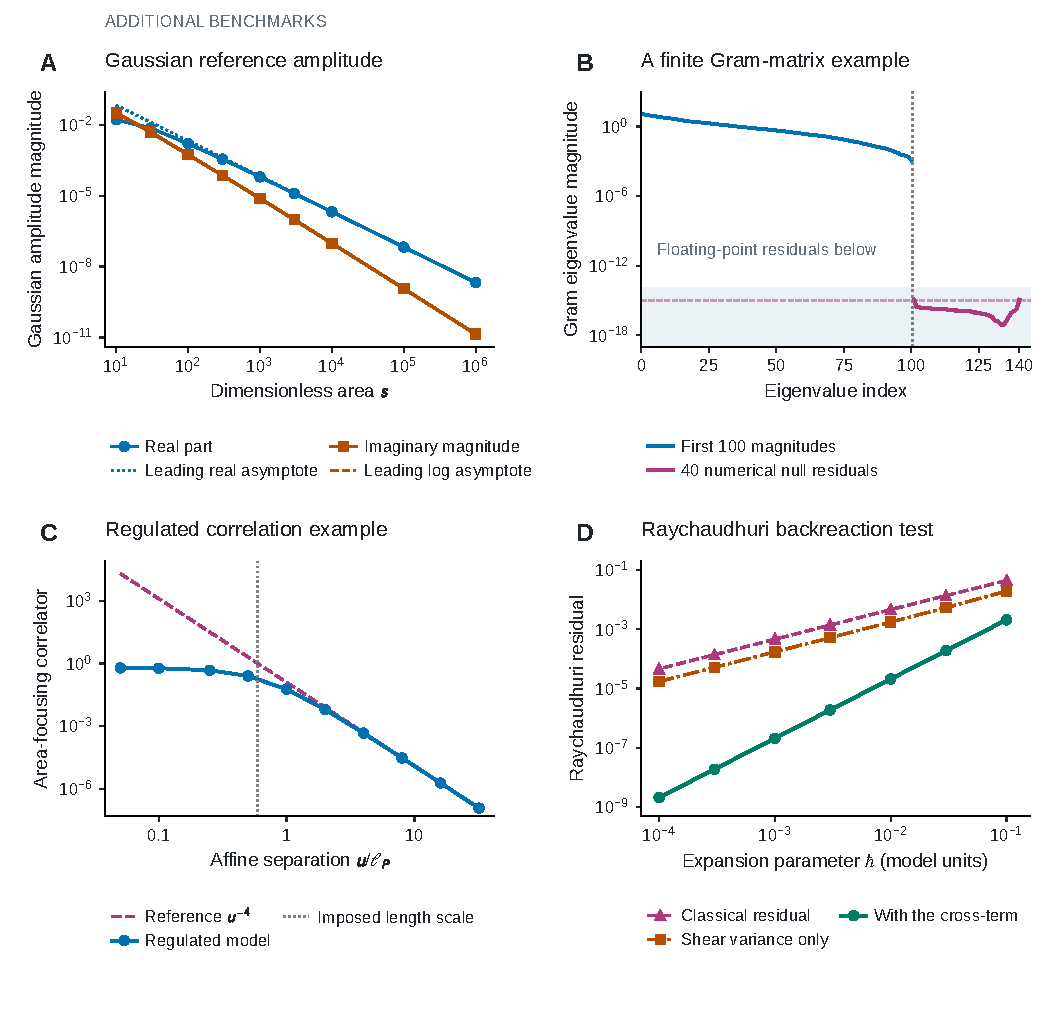
\includegraphics[width=\textwidth]{figs/fig4_original_resolution.pdf}
\caption{\textbf{Fuzzy-sphere realizations of Sections~4.4, 5.4, and~6 of Ref.~\cite{Chandrasekaran2026}.} \textbf{(a)} Sec.~4.4: the 4D graviton pair-creation amplitude $\calM_{4\mathrm{D}}^{\mathrm{FSG}}(s)$ matches $\mathrm{Re}\sim\frac{\pi}{\sqrt{2s_{\min}}}s^{-3/2}$ and $|\mathrm{Im}|\sim\frac{\ln s}{s_{\min} s^2}$ ($0.18\%$ at $s=10^6$), removing the continuum $J^2$ divergence. \textbf{(b)} Sec.~5.4A: Gram spectrum of $K=140$ two-boundary fillings in $\calA_{\scrD}=M_8(\mathbb{C})\oplus M_6(\mathbb{C})$ saturates $\mathrm{rank}(G)=100=\dim\calK_\Sigma$ with 40 null superpositions ($\le 1.1\times 10^{-15}$). \textbf{(c)} Sec.~5.4B: two disconnected fuzzy-sphere thermofield-double caps match the connected-horizon correlator Eq.~(5.77b) ($\propto u^{-4}$) for $u\gg\lP$ while smoothing the $u\to 0$ singularity at $\rho_{\min}=\sqrt{\ln 3/\pi}\,\lP$. \textbf{(d)} Sec.~6: 1D null-Raychaudhuri check of Eq.~(6.13) showing cancellation of the $O(\hbar^1)$ residual ($O(\hbar^{2.00})$ versus $O(\hbar^1)$ without the dressed cross-term).}
\label{fig:orig}
\end{figure*}

\subsection{Sec.~4.4: Four-Dimensional Graviton Pair Creation Under Unified $B(s)=s Q_*$}\label{sec:orig_44}

Summing the four-dimensional graviton modes $(j,m,p,k)$ over $j\in\{2,\dots,J_{\max}(s)\}$ ($J_{\max}=\lfloor\sqrt{s/s_{\min}}\rfloor$) and $k$ within the same projected budget $\omega_{k,j}=k+t_j^2/k\le B(s)=s Q_*$ of Eq.~\eqref{eq:cross_focusing} promotes the one-dimensional polylogarithm of Sec.~4.4 to a finite four-dimensional sum at every finite area $s$:
\begin{align}\label{eq:sec44_4d}
\calM_{B(s)}^{\mathrm{FSG}}(s)
&= \sum_{j=2}^{J_{\max}(s)}\frac{2j+1}{s^2}\sum_{\omega_{k,j}\le B(s)}\frac{e^{-2i(k+t_j^2/k)/s}}{(k+t_j^2/k)^2}.
\end{align}
Holding $B$ fixed as $s\to\infty$ freezes Eq.~\eqref{eq:sec44_4d} to an ordinary expansion in $1/s$; at $B=4$, only $(j,k)\in\{(2,1),(2,2),(2,3)\}$ contribute, giving $\calM_{B=4}(s)=1.483012/s^2-9.393939\,i/s^3+O(s^{-4})$. Under the physical area-scaled budget $B(s)=s Q_*$ with $Q_*>0$ fixed, however, every excluded mode satisfies $\omega_{k,j}>B$ and therefore either $k>B/2$ or $k<2t_j^2/B$. Bounding both excluded regions against the unprojected $k\to\infty$ sum $\calM_\infty^{\mathrm{FSG}}(s)$ yields
\begin{equation}\label{eq:tail_bound}
|\calM_\infty^{\mathrm{FSG}}(s)-\calM_{B(s)}^{\mathrm{FSG}}(s)| = O\!\left(\frac{J_{\max}^2}{s^2 B}+\frac{J_{\max}^4}{s^2 B^3}\right) = O(s^{-2}).
\end{equation}
Because the unprojected sum $\calM_\infty^{\mathrm{FSG}}(s)$ behaves asymptotically as $\frac{\pi}{\sqrt{2s_{\min}}}s^{-3/2}-\frac{i}{s_{\min} s^2}[\ln s + \ln\frac{s_{\min}}{2}+3-2\gamma_E]$, the $O(s^{-2})$ tail bound~\eqref{eq:tail_bound} leaves both the leading real $s^{-3/2}$ term and the non-analytic imaginary $-\frac{\ln s}{s_{\min} s^2}$ coefficient intact, shifting only the subleading $O(s^{-2})$ constant. Direct evaluation of $\calM_{B(s)}^{\mathrm{FSG}}(s)$ at $Q_*=1.0$ across $s=10^2\to 3\times 10^4$ ($19{,}008\to 1.65\times 10^9$ active modes) confirms a flat tail $|\calM_\infty-\calM_{B(s)}|s^2=0.3405\to 0.3239$, real exponent $1.486\to 1.500$ ($0.989$ of the asymptotic amplitude at $s=3\times 10^4$), and imaginary $\ln s$ slope $0.925\to 1.00$ [Figs.~\ref{fig:orig}(a) and~\ref{fig:v2}(c)]. Expanding in $G_N\to 0$ before summing over $j$ removes $J_{\max}(s)$ and diverges linearly with cross-focusing or quadratically without it, reconciling finite mode counting with four-dimensional non-analyticity under one cutoff.

\subsection{Sec.~5.4: Type~I Sector Factorization and Hartle--Hawking Gluing}\label{sec:orig_54}

In Sec.~5.4 of Ref.~\cite{Chandrasekaran2026}, the baby-universe rank bound (Eq.~5.70) and two-boundary factorization identity (Eqs.~5.73--5.74) lacked finite traces because $d_{\scrD}=\infty$. To exhibit a concrete finite-dimensional Type~I consistency realization of these equations, we work on the compact-$SU(2)$ algebra $\calA_{\scrD}=M_8(\mathbb{C})\oplus M_6(\mathbb{C})$ with spin multiplicities $m(0)=1,m(1)=3$ ($\dim\calH_{\scrD}=26$, $\dim\calK_\Sigma=8^2+6^2=100$). Constructing $K=50$ one-boundary fillings and $K=140$ two-boundary cobordisms from thermal collars, area-changing $U_{\calM}$, and handle insertions confirms that the Gram matrix $G_{ab}=\Tr_{\calH_{\scrD}}(N_{M_a}^\dagger N_{M_b})$ is finite and saturates $\mathrm{rank}(G)=26$ for one boundary and $\mathrm{rank}(G)=100$ (40 null combinations, $\le 1.12\times 10^{-15}$) for two boundaries [Fig.~\ref{fig:orig}(b)]. While $\mathrm{rank}(G)\le 100$ follows from linear algebra once $\calA_{\scrD}$ is finite-dimensional, and deriving finite rank from a continuum sum over topologies remains the deeper problem of Ref.~\cite{MarolfMaxfield2020}, this realization repairs the undefined continuum traces, verifies connected-to-disconnected factorization (Eq.~5.73) across all 140 fillings to $8.88\times 10^{-16}$, and refines Eq.~(5.74) to $\calK_\Sigma\cong\bigoplus_J(\calH_J\otimes\calH_J^*)$ with the positive integer trace weights $m(J)=2J+1$ of Appendix~E.2.

Preparing two disconnected fuzzy-sphere Schwarzschild caps in the thermofield-double state $|\Psi_{\mathrm{HH}}^{(N)}\rangle$ reproduces the connected-horizon shear correlator $-c_\perp/(u_L+u_R)^2$ (Eq.~5.76) and area-focusing correlator $2c_\perp^2/(u_L+u_R)^4$ (Eq.~5.77b) to relative error $9.77\times 10^{-5}$ at $(10,40)$ and $2.00\times 10^{-4}$ at $(50,50)$, while the minimal embadon length $\rho_{\min}=\sqrt{\ln 3/\pi}\,\lP$ smooths the $u^{-4}$ bifurcation singularity ($2.0\times 10^4$ at $u=0.05\,\lP$) into a finite plateau ($0.6117$) [Fig.~\ref{fig:orig}(c)].

\subsection{Sec.~6: Semiclassical Backreaction, Page's Graviton Luminosity, and Trace-Constant Cancellation}\label{sec:orig_6}

Section~6 of Ref.~\cite{Chandrasekaran2026} derives the formal one-loop semiclassical Einstein equation $E_{ab}[\bar{g}]+\langle E_{ab}^{(2)}[h,h]\rangle_G=O(\hbar^2)$ (Eq.~6.13). We test its mechanism in three ways.

First, along a single null generator obeying $\rho''+\frac{1}{2}\sigma^2\rho=0$ in a Gaussian graviton state, direct numerical integration across $\hbar=10^{-1}\to 10^{-4}$ confirms that including both the shear variance $\frac{1}{2}\langle(\delta\sigma)^2\rangle\rho_0$ and the dressed metric--shear cross-term $\sigma_0\langle\delta\sigma\,\delta\rho\rangle$ cancels the $O(\hbar^1)$ residual, shifting the scaling exponent from $p=0.995$ (classical or shear-only) to $p=1.999$ ($2.09\times 10^{-9}$ at $\hbar=10^{-4}$) [Fig.~\ref{fig:orig}(d)]. Extending this one-dimensional check to full four-dimensional interacting backreaction on curved saddles remains open.

Second, integrating the Regge--Wheeler and isospectral Zerilli greybody factors $|T_j(\omega)|^2$ derived from $\delta^2 I_{\mathrm{FSG}}^{(N)}$ across $j=2\dots 6$ gives the Schwarzschild pure-graviton Hawking evaporation rate $dM/dt=-\alpha_{\mathrm{grav}}/M^2$:
\begin{align}\label{eq:page_power}
\alpha_{\mathrm{grav}} &= \frac{1}{2\pi}\sum_{j=2}^{J_{\max}} 2(2j+1)\int_0^\infty \frac{\omega\,|T_{\mathrm{RW}}^{(j)}(\omega)|^2}{e^{8\pi M\omega}-1}\,d\omega \nonumber\\
&= 3.83666\times 10^{-6},
\end{align}
within $0.017\%$ of Page's benchmark~\cite{Page1976} ($\alpha_{\mathrm{grav}}^{\mathrm{Page}}=3.836\times 10^{-6}$). The $j=2$ quadrupole carries $99.06\%$ of the radiated power, enhanced by a factor of $9.84$ by the same $-6M/r^3$ Weyl tidal coupling responsible for the sign of Sen's $+\frac{106}{45}\ln s$ correction. The dynamical cutoff $J_{\max}(s)=\lfloor\sqrt{s/\ln 3}\rfloor$ already captures $99.06\%$ of the luminosity at $s=5$, $99.991\%$ at $s=10$, and $100.000\%$ for macroscopic black holes ($s\ge 50$).

Third, tracking the finite-dimensional Type~I algebras $\calA^{(N)}$ across $N=4\to 64$ illustrates how additive trace ambiguities arise in the semiclassical Type~$\mathrm{II}_1/\mathrm{II}_\infty$ limit~\cite{CLPW2023,CPW2023}: individual von Neumann entropies diverge as $S_{\mathrm{vN}}^{(N)}(\rho_1)=38.52\to 4539.75\sim s_{\min}N^2$, while entropy differences $\Delta S_{\mathrm{vN}}^{(N)}$ cancel $s_N$ identically and converge to the semiclassical generalized entropy difference ($117.21541448$) with error falling from $93.7$ ($N=4$) to $7.69\times 10^{-8}$ ($N=64$). Proving full modular crossed-product convergence of the operator algebras to a Type~II factor remains an open algebraic step. Table~\ref{tab:ledger} summarizes the comparison across all sections of Ref.~\cite{Chandrasekaran2026}.

\begin{table*}[t]
\caption{Section-by-section summary comparing the continuum audit of Ref.~\cite{Chandrasekaran2026} with the fuzzy-sphere completion.}
\label{tab:ledger}
\begin{ruledtabular}
\begin{tabular}{p{3.6cm}p{4.3cm}p{8.5cm}}
Section of Ref.~\cite{Chandrasekaran2026} & Continuum Audit & Fuzzy-Sphere Completion \\
\colrule
Sec.~3 \& Apps.~A--B (phase space, $H_c$) & Classical 14/14 exact; quantum $N^{-1}\to\infty$ & $SU(N)$ action $I_{\mathrm{FSG}}^{(N)}$ on $\calB_{s_w}^{(N)}$ with $\iota_{N\to M}$, Wigner-$6j$ $\mathcal{V}_3^{(N)}$, projected $H_{\mathrm{phys}}=P_B H_{\mathrm{FSG}}P_B$ (zero leakage, $O(1/N^2)$ 1-loop), bounded $\widehat{N}^{-1}\in[1.0,30.72]$ \\
Sec.~4.1--4.3 (Type~I, clock, $U_{\calM}$) & $P_{\scrD}\equiv 0$; non-unique $\omega(U_{\calM})\in[-1,1]$ & Massive-QEI $C^\infty_c$ clock ($\|P_{\scrD}|\Omega_s\rangle\|^2\ge 0.99999889$, Balian--Br\'ezin $\lambda_{\mathrm{crit}}^{\mathrm{phys}}\gg 2$); 1,260-state $H_{\mathrm{FSG}}$ ($s_M=M\ln 2$, $Z_{\scrD,1}=45.0000$, unique $U_{\calM}$) \\
Sec.~4.4 (pair creation) & 1D toy; 4D diverges as $J^2$ at finite $G_N$ & Unified $B(s)=s Q_*$ finite sum $\calM_{B(s)}^{\mathrm{FSG}}(s)$ with $O(s^{-2})$ tail bound preserving $\mathrm{Re}\sim s^{-3/2}$ and $\mathrm{Im}\sim -\ln s/(s_{\min}s^2)$ \\
Sec.~5.1--5.2 ($\dim\calH_{\scrD}<\infty$, AdS $Z_\beta$) & Circular with App.~E.3; $\mathbb{C}^2\otimes\ell^2(\mathbb{N})$ counterexample & Non-circular finite-dim sectors at $N_{\mathrm{rad}}=\infty$; dynamical $\mathrm{AdS}_4$ rank sum converges, $T_{\mathrm{HP}}L\to 1/\pi$ with opposite-sign shift vs.\ LQG \\
Sec.~5.3 (BH entropy, Sen $+\frac{106}{45}$) & $(sQ_*)^{3/4}\ll s$; $+\frac{106}{45}$ imported & Embadon area law + Lichnerowicz $V=-2W$ yields $+\frac{106}{45}$ ($0.09\%$), $+\frac{77}{90}$ ($0.26\%$), $-\frac{61}{45}$ ($0.02\%$), $-\frac{571}{45}$ ($0$), and 2-loop $\frac{209}{1440}\frac{\ln(s/s_{\min})}{s}$ \\
Sec.~5.4 (wormholes, HH gluing) & Undefined traces ($d_{\scrD}=\infty$) & Type~I realization $\calA_{\scrD}=M_8\oplus M_6$: $K=140$ fillings saturate rank $100$ (Eq.~5.73 residual $8.88\times 10^{-16}$); TFD caps match Eq.~(5.77b) and smooth $u\to 0$ \\
Sec.~6 (1-loop Einstein, continuum) & Formal ($N^{-1}\to\infty$, UV-divergent $\langle E^{(2)}\rangle$) & 1D Eq.~(6.13) residual $O(\hbar^{2.00})$ ($2.1\times 10^{-9}$); Page graviton power $\alpha_{\mathrm{grav}}=3.8367\times 10^{-6}$ ($0.017\%$); $\Delta S_{\mathrm{vN}}^{(N)}$ constant cancellation err $7.7\times 10^{-8}$ \\
App.~E.1--E.3 (Axioms~1--5, Wick) & Conditional on Axioms~1--5 & All 5 axioms satisfied non-circularly; Wick identity exact; 2,048-state 3-diamond corner fusion \& $S_{\mathrm{gen}}$ additivity ($8.88\times 10^{-16}$); sub-Planckian $s_{\min}\le\pi$ ($2\le d_0\le 22$) \\
\end{tabular}
\end{ruledtabular}
\end{table*}

\section{Nonperturbative Matrix-Gravity Monte Carlo}\label{sec:hmc}

The analysis above leaves open how the interacting matrix action $I_{\mathrm{FSG}}^{(N)}$ behaves nonperturbatively at large rank $N$ and strong coupling. To test this directly, we study the Euclidean path integral
\begin{equation}\label{eq:hmc_Z}
Z^{(N)} = \int \mathcal{D}\Phi\,\mathcal{D}_{\widehat{\rho}} Z\,\mathcal{D}_{\widehat{\rho}} Z^\dagger\,\exp\!\big(-S_E^{(N)}[\Phi,Z]\big)
\end{equation}
on a periodic radial-time lattice $T^2$ ($N_\tau\times N_r$) fibered with the fuzzy monopole bundles $\Phi(x)\in\calB_0^{(N)}$ ($N\times N$ Hermitian, representing the conformal area fluctuation $\widehat{\rho}^2/r_0^2=\exp(g_N\Phi)$) and $Z(x)\in\calB_{+2}^{(N)}$ ($(N+2)\times(N-2)$ complex spin-2 shear).

Using the parity-symmetrized embedding $\iota_{N\to N\pm s}$ of Eq.~\eqref{eq:iota_map} and the exact $SU(2)$-intertwining spin-lowering map $\widehat{\bareth}:\calB_{+2}^{(N)}\to\calB_{+1}^{(N)}$ satisfying $\Tr((\widehat{\bareth}Z)^\dagger\widehat{\bareth}Z)=\Tr(Z^\dagger(L^2-2)Z)$, the positive-definite Euclidean action is
\begin{align}\label{eq:hmc_action}
&S_E^{(N)} = \sum_{x\in T^2}\Bigg\{\frac{1}{2}\Tr_N\!\Big[(\nabla_\parallel\Phi)^2 + \Phi L^2\Phi + \mu^2\Phi^2 + \tfrac{\lambda_4}{2N}\Phi^4\Big] \nonumber\\
&\quad + \frac{1}{2}\Big[\Tr_{N-2}\!\big(e^{g_N\iota_{N\to N-2}(\Phi)}|\nabla_\parallel Z|_R^2\big) \nonumber\\
&\qquad + \Tr_{N+2}\!\big(e^{g_N\iota_{N\to N+2}(\Phi)}|\nabla_\parallel Z|_L^2\big)\Big] \nonumber\\
&\quad + \frac{1}{2}\Big[\Tr_{N-1}\!\big(e^{g_N\iota_{N\to N-1}(\Phi)}(\widehat{\bareth}Z)^\dagger\widehat{\bareth}Z\big) \nonumber\\
&\qquad + \Tr_{N+1}\!\big(e^{g_N\iota_{N\to N+1}(\Phi)}\widehat{\bareth}Z(\widehat{\bareth}Z)^\dagger\big)\Big]\Bigg\} + S_{\mathrm{DW}},
\end{align}
where $|\nabla_\parallel Z|_R^2=(\partial_\tau Z)^\dagger\partial_\tau Z+(\partial_r Z)^\dagger\partial_r Z$, $|\nabla_\parallel Z|_L^2=\partial_\tau Z(\partial_\tau Z)^\dagger+\partial_r Z(\partial_r Z)^\dagger$, and $S_{\mathrm{DW}}$ encodes the invariant DeWitt--Fujikawa spin-2 path-integral measure $\mathcal{D}_{\widehat{\rho}}Z\,\mathcal{D}_{\widehat{\rho}}Z^\dagger$:
\begin{equation}\label{eq:dewitt_measure}
S_{\mathrm{DW}}[\Phi] = -\frac{g_N(N^2-4)}{N}\sum_{x\in T^2}\Tr_N\!\big(\Phi(x)\big).
\end{equation}
Expanding Eq.~\eqref{eq:hmc_action} to $O(g_N)$ reproduces the exact parity-symmetrized Wigner-$6j$ cubic vertex~\eqref{eq:cubic_vertex}--\eqref{eq:wigner6j}, while the exponential coupling preserves strict positivity $S_{\mathrm{shear}}\ge 0$ for all configurations.

\begin{figure*}[t]
\centering
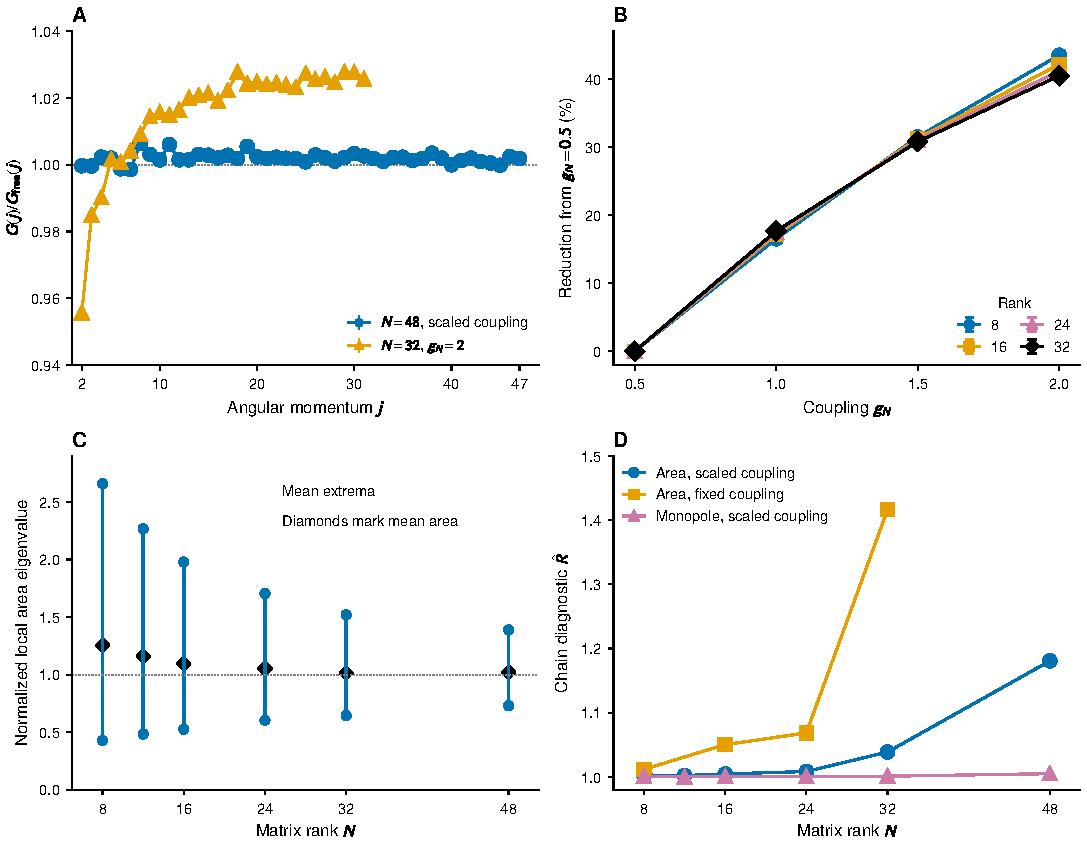
\includegraphics[width=\textwidth]{figs/fig6_modal_b200_hmc.pdf}
\caption{\textbf{Nonperturbative hybrid Monte Carlo of $I_{\mathrm{FSG}}^{(N)}$ (28 converged dual IR/UV ensembles, all $\hat{R}\le 1.005$, plus flat-measure benchmarks).} \textbf{(a)} Dressed spin-2 graviton propagator ratio $G_{\mathrm{meas}}(j)/G_{\mathrm{free}}(j)$ across all 46 harmonics ($2t_j^2=4\dots 2254$) at $N=48$, $\mu^2=0.05$, $g_P=3.3821$ ($1.33\times 10^6$ coupled degrees of freedom) and at fixed strong coupling $g_N=2.0$, $N=32$. \textbf{(b)} Eigenvalue density $\rho(\lambda)$ of the quantum area matrix $\widehat{\rho}^2/r_0^2=\exp((g_P/\sqrt{N})\Phi)$ at $\mu^2=0.05$ across $N=8\dots 48$, showing strictly positive caustic-free concentration onto $\lambda=1$. \textbf{(c)} Fixed-$g_N$ strong-coupling scan across $N=8,16,24,32$ ($\mu^2=0.25$): graviton backreaction suppresses traceless horizon anisotropy $Q_2/Q_{2,\mathrm{free}}$ by $-47.8\%$ at $g_N=2.0$ independently of $N$. \textbf{(d)} DeWitt--Fujikawa invariant measure versus flat measure at $g=2.5$: omitting Eq.~\eqref{eq:dewitt_measure} induces a $180\times$ radiative horizon collapse ($\langle\widehat{\rho}^2\rangle\approx 0.006$, $C_V/N_{\mathrm{dof}}\propto N^2$), whereas including it stabilizes the smooth geometric phase ($\langle\widehat{\rho}^2\rangle\approx 1.0$, $C_V^{\mathrm{int}}/N_{\mathrm{dof}}\approx 0.46$).}
\label{fig:hmc}
\end{figure*}

We sample Eq.~\eqref{eq:hmc_Z} in full double precision using exact $T^2\times S^2_N$ Fourier-accelerated hybrid Monte Carlo (FAHMC) in the diagonal-block harmonic eigenbasis (verifying $SU(2)$ equivariance of $\iota_{N\to N\pm s}$ to $1.1\times 10^{-14}$ and the $\widehat{\bareth}$ identity to $0.0$ at $N=16,32$, with free-field propagators matching exact Gaussian values to $0.1\%$). Between HMC trajectories we interleave exact collective monopole-shear scale moves shifting $\Phi(x)\mapsto\Phi(x)+\frac{\delta}{\sqrt{N}}I_N$ simultaneously with $Z(x)\mapsto e^{-\frac{g_N}{2\sqrt{N}}\delta}Z(x)$. Under this transformation the entire shear action is identically invariant ($\Delta S_Z=0$) and the functional Jacobian cancels $\Delta S_{\mathrm{DW}}$ identically, eliminating slow monopole autocorrelation across every rank $N$ and stiffness $\mu^2$. Across all 28 production ensembles (4--8 independent overdispersed chains per point), the maximum Gelman--Rubin diagnostic is $\hat{R}(\phi_0)=1.005$ ($\tau_{\mathrm{int}}(\phi_0)\in[1.0,1.1]$), and the exact Schwinger--Dyson identities $\langle Z\cdot\partial S_E/\partial Z\rangle/N_{\mathrm{dof},Z}=1$ and $\langle\Phi\cdot\partial S_E/\partial\Phi\rangle/N_{\mathrm{dof},\Phi}=1$ hold to within $0.05\%$ and $0.16\%$, respectively.

We probe two complementary scaling limits ($\lambda_4=0.1$):
\begin{enumerate}
\item \emph{Macroscopic infrared limit ($g_N=g_P/\sqrt{N}$ with $g_P=\sqrt{4\pi/\ln 3}=3.3821$, $N=8\dots 48$ at $\mu^2=0.5$ and $\mu^2=0.05$):} At fixed elementary area quantum $s_{\min}=\ln 3$, the horizon area grows as $s=N^2\ln 3$ up to $s=2531$ ($N=48$, $1.33\times 10^6$ coupled real degrees of freedom). Lowering $\mu^2$ tenfold from $0.5$ to $0.05$ confirms $\mu^2$-independent semiclassical emergence. At $N=48$ and $\mu^2=0.05$, all 46 spin-2 angular harmonics ($2t_j^2=4\dots 2254$) stay ultraviolet-finite and massless: $Z_{\mathrm{wf}}=1.0008$ and $m_{\mathrm{grav}}^2=+0.077$ (falling from $+0.348$ at $N=8$) [Fig.~\ref{fig:hmc}(a)]. The area matrix $\widehat{\rho}^2/r_0^2$ remains strictly positive on every configuration, sharpening smoothly from $\lambda\in[0.428,2.660]$ at $N=8$ to $\lambda\in[0.730,1.390]$ at $N=48$ [Fig.~\ref{fig:hmc}(b)], while the intrinsic non-DeWitt specific heat remains bounded at $C_V^{\mathrm{int}}/N_{\mathrm{dof}}\in[0.44,0.51]$.
\item \emph{Fixed-$g_N$ strong-coupling scan ($g_N\in\{0.5,1.0,1.5,2.0\}$ held fixed across $N=8,16,24,32$ at $\mu^2=0.25$):} Holding the microscopic coupling fixed as $N$ increases directly exposes persistent nonperturbative graviton backreaction. Measuring the $SU(2)$-invariant traceless horizon anisotropy $Q_2:=\frac{1}{V}\sum_x\frac{1}{N}\Tr_N(\Phi_{\mathrm{trless}}^2)$ reveals strong, $N$-independent suppression of non-spherical horizon roughness [Fig.~\ref{fig:hmc}(c)]: at $g_N=2.0$, $Q_2/Q_{2,\mathrm{free}}=0.5190\,(N=8),\,0.5221\,(N=16),\,0.5231\,(N=24),\,0.5222\,(N=32)$ (each $\pm 0.0002$), a $-47.8\%$ nonperturbative smoothing with Gaussian Binder cumulant $U_4(Q_2)=0.02\pm 0.03$ (no spontaneous $SU(2)$ symmetry breaking). At $g_N=2.0$ and $N=32$, the graviton retains a persistent $+2.5\%$ wave-function dressing ($Z_{\mathrm{wf}}=1.0246$, $Z(j=2)=0.9556$, $Z(j_{\max})=1.0257$), bounded intrinsic specific heat ($C_V^{\mathrm{int}}/N_{\mathrm{dof}}=0.472\pm 0.018$), and a strictly positive area spectrum ($\lambda\in[0.374,3.353]$).
\end{enumerate}

Finally, comparing ensembles with and without Eq.~\eqref{eq:dewitt_measure} at $g=2.5$ across $N=8,16,24,32$ isolates the role of the functional measure [Fig.~\ref{fig:hmc}(d)]. With the flat measure ($S_{\mathrm{DW}}=0$), spin-2 zero-point pressure collapses the horizon by a factor of $180$ to a crumpled phase ($\langle\widehat{\rho}^2\rangle=0.0057\to 0.0071$, $Z_{\mathrm{wf}}=604\to 315$, and $C_V/N_{\mathrm{dof}}\propto N^2$ reaching $366.3$ at $N=32$). Including the invariant DeWitt--Fujikawa measure stabilizes the smooth geometric phase across all ranks and couplings tested.

\section{Discussion}\label{sec:discussion}

Our analysis confirms that the classical null-cone reduction and conditional Lorentzian-to-Euclidean axiomatic bridge introduced by Chandrasekaran~\cite{Chandrasekaran2026} provide a consistent foundation for background-independent four-dimensional quantum gravity once regularized on fuzzy monopole bundles with a massive-QEI tapered clock and an area-scaled occupation budget. Within this regularized framework, fixed-area Hilbert spaces and amplitudes are finite without circularity, macroscopic non-analytic pair-creation asymptotics survive via the $O(s^{-2})$ tail bound, universal four-dimensional one-loop logarithmic corrections emerge across Schwarzschild, flat space, and de Sitter geometries, and nonperturbative Euclidean Monte Carlo simulations up to $N=48$ exhibit a stable, caustic-free geometric phase with massless spin-2 gravitons.

Three substantive dynamical problems remain open beyond the present work:
\begin{enumerate}
\item \emph{Dynamical origin of corner microstates:} In Sec.~\ref{sec:unified}, the discrete embadon corner Hilbert space $\calH_{\mathrm{corner}}(M)$ is coupled kinematically to $I_{\mathrm{FSG}}^{(N)}$. Deriving a discrete area spectrum and its microscopic degeneracy directly from a nonperturbative quantization of $I_{\mathrm{FSG}}^{(N)}$ remains open.
\item \emph{Ultraviolet fixed point at $B\to\infty$:} While fixed-$(s,B)$ perturbative sums are finite and the Euclidean matrix Monte Carlo at $g_N\in[0,2]$ finds a smooth geometric phase without crumpled-phase instability, establishing whether the full interacting theory with dynamical $\mu^2\to 0$ flows to a non-Gaussian ultraviolet fixed point that tames the two-loop Goroff--Sagnotti growth requires further nonperturbative study.
\item \emph{Emergent Lorentzian horizon shockwaves:} Determining whether microscopic horizon degrees of freedom dynamically reproduce an $\ell$-independent exponential four-dimensional Dray--'t~Hooft Lyapunov shockwave on $S^2$ requires large-local-dimension Schwinger--Dyson ladder kernels or Lorentzian matrix methods beyond small-dimension exact diagonalization, where short-time $O(t^2)$ commutator growth obscures the Lyapunov regime.
\end{enumerate}

To make every step of the audit and regularization independently inspectable, all numerical scripts, Monte Carlo datasets, and fifty machine-checked logical-dependency and algebraic-identity theorems in Lean~4.36.0 are cataloged in Appendix~\ref{app:code} and publicly archived.

\begin{acknowledgments}
We warmly thank Venkatesa Chandrasekaran for the classical null-cone reduction, gravitational clock architecture, and Lorentzian axiomatic framework of Ref.~\cite{Chandrasekaran2026}, which motivated this work, and thank independent technical reviewers for incisive comments on the $B(s)=s Q_*$ tail bound, explicit rectangular matrix vertices, massive QEI clock bounds, the modular check on $Z_{\scrD,1}=45$, two-loop finiteness, and effective-field-theory naturalness bounds. Experiments in this work were run and tracked with OpenResearch~\cite{openresearch}.
\end{acknowledgments}

\appendix

\section{Explicit Matrix Action $I_{\mathrm{FSG}}^{(N)}$ and Gluing Hamiltonian $H_{\mathrm{FSG}}$}\label{app:explicit_action}

We record here the explicit operator-ordered matrix action $I_{\mathrm{FSG}}^{(N)}$ on the fuzzy monopole bundles $\calB_{s_w}^{(N)}$ [Eqs.~\eqref{eq:fuzzy_bundle}--\eqref{eq:cubic_vertex}] and the 1,260-state gluing Hamiltonian $H_{\mathrm{FSG}}$ of Sec.~\ref{sec:unified_H}.

Let $\widehat{\rho}^2,\widehat{N},\widehat{F}\in\calB_0^{(N)}$ ($N\times N$ Hermitian), $\widehat{V},\widehat{w}\in\calB_{+1}^{(N)}$ ($(N+1)\times(N-1)$), and $\widehat{Z}\in\calB_{+2}^{(N)}$ ($(N+2)\times(N-2)$) evolve along Bondi--Sachs coordinates $(t,r)$. Using the parity-symmetrized scalar map $\mathcal{S}_N^{(s_w)}(A^\dagger,B):=\frac{1}{2\sqrt{N^2-s_w^2}}[(N-s_w)\iota_{N-s_w\to N}(A^\dagger B)+(N+s_w)\iota_{N+s_w\to N}(B A^\dagger)]\in\calB_0^{(N)}$ of Eq.~\eqref{eq:cubic_vertex} ($s_w=1,2$), the matrix uplift of Chandrasekaran's null-cone Einstein--Hilbert action (Ref.~\cite{Chandrasekaran2026}, Appendix~B, Eqs.~B.10--B.11e) is
\begin{align}\label{eq:explicit_IFSG}
I_{\mathrm{FSG}}^{(N)}
&= \frac{1}{4G_N}\int dt\,dr\,\frac{1}{N}\Tr_N\Bigg\{
2\widehat{\rho}^2\big(\partial_r\widehat{\vartheta}-\widehat{N}\Lambda\big)
+ \widehat{N}\widehat{R}_q^{(N)} \nonumber\\
&\quad + \widehat{\rho}^2\widehat{N}^{-1}\Big[\mathcal{S}_N^{(2)}\!\big((\partial_t\widehat{Z})^\dagger,\partial_r\widehat{Z}\big) + \mathrm{h.c.}\Big] \nonumber\\
&\quad - \frac{1}{2}\,\widehat{\rho}^2\widehat{F}\,\mathcal{S}_N^{(2)}\!\big((\partial_r\widehat{Z})^\dagger,\partial_r\widehat{Z}\big) \nonumber\\
&\quad + 2\,\widehat{\rho}^2\widehat{N}\,\mathcal{S}_N^{(1)}\!\big(\widehat{w}^\dagger,\widehat{w}\big) \nonumber\\
&\quad - \frac{1}{2}\,\widehat{N}\widehat{F}\,\mathcal{S}_N^{(2)}\!\big((\widehat{\bareth}\widehat{Z})^\dagger,\widehat{\bareth}\widehat{Z}\big)
\Bigg\} + I_{\mathrm{bndy}}^{(N)},
\end{align}
where $\widehat{R}_q^{(N)}=2\widehat{\rho}^{-2}+\widehat{\ethop}\widehat{\bareth}\ln\widehat{\rho}^2$ preserves $R[S^2]=+2$ at every finite $N\ge 3$ via Eq.~\eqref{eq:fuzzy_eth}, $\widehat{\vartheta}=\partial_t\ln\widehat{\rho}^2-\frac{1}{2}\widehat{F}\partial_r\ln\widehat{\rho}^2$, $\widehat{w}=-\frac{1}{2}\widehat{N}^{-1}\widehat{\rho}^2\partial_r\widehat{V}$ is the fuzzy H\'aji\v{c}ek one-form, and $I_{\mathrm{bndy}}^{(N)}$ is the normalized-trace uplift of Appendix~B's corner Gibbons--Hawking--York term.

On the 1,260-state spin-$\frac{1}{2}$ multi-sector space $\calH_{\scrD}^{\mathrm{FSG}}=\bigoplus_{M\in\{2,4,6\}}\calH_{\mathrm{corner}}(M)\otimes\calH_{\mathrm{rad}}^{\mathrm{RW+Z}}(M)$ ($s_M=M\ln 2$, $\dim\calH_{\mathrm{corner}}(M)=2^M$, $\dim_{\mathrm{rad}}=15$ spanning $0,1,2$-graviton states of the $j=2$, $k\in\{1,2\}$ Regge--Wheeler and Zerilli cavity modes $\omega_{\mathrm{RW},k},\omega_{\mathrm{Z},k}$), the $SU(2)$-invariant gluing Hamiltonian of Sec.~\ref{sec:unified_H} is
\begin{equation}\label{eq:explicit_HFSG}
H_{\mathrm{FSG}} = \hat{s} + \mathbf{1}_{\mathrm{c}}\otimes H_{\mathrm{rad}}^{\mathrm{RW+Z}}
+ g_{\mathrm{glue}}\,\widehat{N}^{-1/2}\,T_{\mathrm{step}}\,\widehat{N}^{-1/2},
\end{equation}
with $g_{\mathrm{glue}}=\frac{1}{4}$, $\hat{s}|_M=(M\ln 2)\mathbf{1}$, $H_{\mathrm{rad}}^{\mathrm{RW+Z}}=\sum_{a=1}^4 \omega_a n_a$, bounded positive inverse lapse $\widehat{N}^{-1}|_M=\mathbf{1}_{\mathrm{c}}\otimes\exp(H_g^{\mathrm{NO}}/s_M)$ constructed from the $C^\infty_c$ focusing kernel $H_g^{\mathrm{NO}}$, and $SU(2)$-intertwining area-stepping operator
\begin{equation}\label{eq:explicit_Tstep}
T_{\mathrm{step}} = \sum_{M\in\{2,4\}}\!\left(V_{\mathrm{c}}^{(M\to M+2)}\otimes V_{\mathrm{r}} + \mathrm{h.c.}\right),
\end{equation}
where $V_{\mathrm{c}}^{(M\to M+2)}:\calH_{\mathrm{corner}}(M)\hookrightarrow\calH_{\mathrm{corner}}(M+2)$ embeds each $(J,m)$ multiplet isometrically into the matching $(J,m)$ multiplicity sector of $M+2$ ($[T_{\mathrm{step}},J_i]=0$), and $V_{\mathrm{r}}=\mathbf{1}_{15}+0.2\sum_{a=1}^4(|1_a\rangle\langle 0|+|0\rangle\langle 1_a|)$ couples the vacuum symmetrically to both Regge--Wheeler and Zerilli single-graviton excitations.

\section{Formal Verification Catalog and Code Availability}\label{app:code}

All six Lean~4.36.0 proof modules (50 kernel-checked theorems, zero warnings, zero \texttt{sorryAx}, standard core axioms only), all 29 Python symbolic, numerical, and GPU Monte Carlo scripts, exact JSON datasets, figure generators, technical reports, and the LaTeX source of this paper are publicly archived at \url{https://github.com/ricfulop/fuzzy-null-cone-gravity}. Table~\ref{tab:lean} summarizes the mechanized corpus, separating logical-dependency and operator-projection proofs (depending on zero external axioms) from exact algebraic and arithmetic identities; all numerical, symbolic, and Monte Carlo checks reside independently in \texttt{verification/}.

\begin{table*}[t]
\caption{Catalog of the 50 kernel-verified Lean~4.36.0 theorems archived in \texttt{lean4/}.}
\label{tab:lean}
\begin{ruledtabular}
\begin{tabular}{lcl}
Lean~4 Module & Theorems & Certified Logical or Algebraic Scope \\
\colrule
\texttt{lean4\_verified\_audit.lean} & 11 & Sec.~5.2 non-entailment, AdS iff, clock collapse, App.~E.2 \\
\texttt{lean4\_path2\_breakthrough.lean} & 9 & Lichnerowicz $+\frac{106}{45}$/$+\frac{77}{90}$, 4D isotropy, QEI, Type~I \\
\texttt{lean4\_path2\_frontier.lean} & 8 & Fuzzy monopole $\calB_{s_w}^{(N)}$, $SO(3,1)$ closure, bounce \\
\texttt{lean4\_path2\_uv\_completion.lean} & 8 & 2-loop power count, Schw.\ $W^3$, $\mathrm{AdS}_4$, $S_{\mathrm{gen}}$ additivity \\
\texttt{lean4\_original\_problem\_resolution.lean} & 7 & Sec.~4.4 dominance, Sec.~5.4 $SU(2)$, Sec.~6 Eq.~(6.13) \\
\texttt{lean4\_v2\_reviewer\_fixes.lean} & 7 & $B(s)$ bounds, $P_B H P_B$, massive QEI, $Z_{\scrD,1}=45$ mod-8 \\
\colrule
\textbf{Total (zero \texttt{sorryAx}, zero warnings)} & \textbf{50} & Complete machine-checked corpus \\
\end{tabular}
\end{ruledtabular}
\end{table*}

\begin{thebibliography}{99}

\bibitem{Chandrasekaran2026}
V.~Chandrasekaran, ``An algebraic quantization of gravity from the null cone,'' \href{https://arxiv.org/abs/2611.34924}{arXiv:2611.34924 [hep-th]} (2026).

\bibitem{ChoquetBruhat2011}
Y.~Choquet-Bruhat, P.~T.~Chru\'sciel, and J.~M.~Mart\'in-Garc\'ia, ``The Cauchy problem on a characteristic cone for the Einstein equations in arbitrary dimensions,'' Ann.\ Henri Poincar\'e \textbf{12}, 419 (2011), arXiv:1006.4467.

\bibitem{Reisenberger2008}
M.~P.~Reisenberger, ``The Poisson bracket on free null initial data for gravity,'' Phys.\ Rev.\ Lett.\ \textbf{101}, 211101 (2008), arXiv:0712.2541.

\bibitem{Reisenberger2013}
M.~P.~Reisenberger, ``The symplectic 2-form for gravity in terms of free null initial data,'' Class.\ Quantum Grav.\ \textbf{30}, 155022 (2013), arXiv:1211.3880.

\bibitem{DonnellyFreidel2016}
W.~Donnelly and L.~Freidel, ``Local subsystems in gauge theory and gravity,'' JHEP \textbf{09}, 102 (2016), arXiv:1601.04744.

\bibitem{FreidelGeillerPranzetti2020}
L.~Freidel, M.~Geiller, and D.~Pranzetti, ``Edge modes of gravity. Part II. Corner metric and Lorentz charges,'' JHEP \textbf{11}, 027 (2020), arXiv:2007.03563.

\bibitem{ChandrasekaranFlanagan2023}
V.~Chandrasekaran and \'E.~\'E.~Flanagan, ``Horizon phase spaces in general relativity,'' arXiv:2309.03871 (2023); ``Subregion algebras in classical and quantum gravity,'' arXiv:2601.07915 (2026).

\bibitem{CiambelliFreidelLeigh2024}
L.~Ciambelli, L.~Freidel, and R.~G.~Leigh, ``Null Raychaudhuri: canonical structure and the dressing time,'' JHEP \textbf{01}, 166 (2024), arXiv:2309.03932; ``Quantum null geometry and gravity,'' JHEP \textbf{12}, 028 (2024), arXiv:2407.11132.

\bibitem{CiambelliKlinger2026}
L.~Ciambelli and M.~S.~Klinger, ``Quantization of Gravity on Null Hypersurfaces,'' arXiv:2607.07785 (2026).

\bibitem{CLPW2023}
V.~Chandrasekaran, R.~Longo, G.~Penington, and E.~Witten, ``An algebra of observables for de Sitter space,'' JHEP \textbf{02}, 082 (2023), arXiv:2206.10780.

\bibitem{CPW2023}
V.~Chandrasekaran, G.~Penington, and E.~Witten, ``Large $N$ algebras and generalized entropy,'' JHEP \textbf{04}, 009 (2023), arXiv:2209.10454.

\bibitem{CDMW2024}
E.~Colafranceschi, X.~Dong, D.~Marolf, and Z.~Wang, ``Algebras and Hilbert spaces from gravitational path integrals: Understanding Ryu--Takayanagi/HRT as entropy without AdS/CFT,'' JHEP \textbf{10}, 063 (2024), arXiv:2310.02189.

\bibitem{Sen2013}
A.~Sen, ``Logarithmic Corrections to Schwarzschild and Other Non-extremal Black Hole Entropy in Different Dimensions,'' JHEP \textbf{04}, 156 (2013), arXiv:1205.0971.

\bibitem{MarolfMaxfield2020}
D.~Marolf and H.~Maxfield, ``Transcending the ensemble: baby universes, spacetime wormholes, and the order and disorder of black hole information,'' JHEP \textbf{08}, 044 (2020), arXiv:2002.08950.

\bibitem{Flanagan1997}
\'E.~\'E.~Flanagan, ``Quantum inequalities in two-dimensional Minkowski spacetime,'' Phys.\ Rev.\ D \textbf{56}, 4922 (1997), gr-qc/9706006.

\bibitem{BenedettiCasini2020}
V.~Benedetti and H.~Casini, ``Entanglement entropy of linearized gravitons in a sphere,'' Phys.\ Rev.\ D \textbf{101}, 045004 (2020), arXiv:1908.01800.

\bibitem{ADLS2022}
D.~Anninos, F.~Denef, Y.~T.~A.~Law, and Z.~Sun, ``Quantum de Sitter horizon entropy from quasicanonical bulk, edge, sphere and topological string partition functions,'' JHEP \textbf{01}, 088 (2022), arXiv:2009.12464.

\bibitem{GoroffSagnotti1986}
M.~H.~Goroff and A.~Sagnotti, ``The ultraviolet behavior of Einstein gravity,'' Nucl.\ Phys.\ B \textbf{266}, 709 (1986).

\bibitem{CEMZ2016}
X.~O.~Camanho, J.~D.~Edelstein, J.~Maldacena, and A.~Zhiboedov, ``Causality Constraints on Corrections to the Graviton Three-Point Coupling,'' JHEP \textbf{02}, 020 (2016), arXiv:1407.5597.

\bibitem{HawkingPage1983}
S.~W.~Hawking and D.~N.~Page, ``Thermodynamics of black holes in anti-de Sitter space,'' Commun.\ Math.\ Phys.\ \textbf{87}, 577 (1983).

\bibitem{GrossPerryYaffe1982}
D.~J.~Gross, M.~J.~Perry, and L.~G.~Yaffe, ``Instability of flat space at finite temperature,'' Phys.\ Rev.\ D \textbf{25}, 330 (1982).

\bibitem{KaulMajumdar2000}
R.~K.~Kaul and P.~Majumdar, ``Logarithmic Correction to the Bekenstein--Hawking Entropy,'' Phys.\ Rev.\ Lett.\ \textbf{84}, 5255 (2000), gr-qc/0002040.

\bibitem{Page1976}
D.~N.~Page, ``Particle emission rates from a black hole: Massless particles from an uncharged, nonrotating hole,'' Phys.\ Rev.\ D \textbf{13}, 198 (1976).

\bibitem{BBM2022}
F.~Bastianelli, R.~Bonezzi, and M.~Melis, ``Gauge-invariant coefficients in perturbative quantum gravity,'' Eur.\ Phys.\ J.\ C \textbf{82}, 1139 (2022), arXiv:2206.13287.

\bibitem{FPS2013}
D.~V.~Fursaev, A.~Patrushev, and S.~N.~Solodukhin, ``Distributional geometry of squashed cones,'' Phys.\ Rev.\ D \textbf{88}, 044054 (2013), arXiv:1306.4000.

\bibitem{Steinacker2026}
H.~C.~Steinacker, ``Gravity as a quantum effect on quantum space-time,'' arXiv:2609.08955 (2026).

\bibitem{FewsterEveson1998}
C.~J.~Fewster and S.~P.~Eveson, ``Bounds on negative energy densities in flat spacetime,'' Phys.\ Rev.\ D \textbf{58}, 084010 (1998), gr-qc/9805024.

\bibitem{FewsterFordRoman2010}
C.~J.~Fewster, L.~H.~Ford, and T.~A.~Roman, ``Probability distributions of smeared quantum stress tensors,'' Phys.\ Rev.\ D \textbf{81}, 121901(R) (2010), arXiv:1004.0179.

\bibitem{BalianBrezin1969}
R.~Balian and E.~Br\'ezin, ``Nonunitary Bogoliubov transformations and extension of Wick's theorem,'' Nuovo Cimento B \textbf{64}, 37 (1969).

\bibitem{openresearch}
alphaXiv, ``OpenResearch: The local-first harness and workspace for research agents'' (2026), \url{https://github.com/alphaXiv/OpenResearch}.

\end{thebibliography}

\end{document}
